\documentclass[9pt,a4paper]{extarticle}

\usepackage[T1]{fontenc}
\usepackage[utf8]{inputenc}
\usepackage{lmodern}
\usepackage[margin=1.25cm,top=1.75cm,bottom=1.35cm,headheight=12pt,headsep=7pt,footskip=12pt]{geometry}
\usepackage{amsmath,amssymb}
\usepackage{graphicx}
\usepackage{booktabs}
\usepackage{array}
\usepackage{longtable}
\usepackage{tabularx}
\usepackage{float}
\usepackage{caption}
\usepackage{subcaption}
\usepackage{xcolor}
\usepackage[hidelinks]{hyperref}
\usepackage{url}
\usepackage{enumitem}
\usepackage{fancyhdr}
\usepackage{titlesec}
\usepackage{multicol}


\hypersetup{hidelinks,pdftitle={Cellular Network Design in Bangladesh},
            pdfauthor={CSE-4103 Case Study}}

\captionsetup{font=footnotesize,labelfont=bf,skip=3pt}
\setlength{\parindent}{0pt}
\setlength{\parskip}{1.5pt}
\renewcommand{\arraystretch}{1.05}

\titleformat{\section}{\normalfont\large\bfseries}{\thesection}{0.6em}{}
\titlespacing{\section}{0pt}{7pt}{3pt}
\titlespacing{\subsection}{0pt}{5pt}{2pt}
\titleformat{\subsection}{\normalfont\normalsize\bfseries}{\thesubsection}{0.5em}{}

\pagestyle{fancy}
\fancyhf{}
\renewcommand{\headrulewidth}{0.4pt}
\fancyhead[L]{\footnotesize CSE-4103 Cellular and Wireless Communication}
\fancyhead[R]{\footnotesize BAUET, Summer 2026}
\fancyfoot[C]{\footnotesize\thepage}
\fancyfoot[R]{\scriptsize Case study: Cellular Network Design in Bangladesh}

% Link labels must be breakable: \nolinkurl breaks at / . - _ and is coloured.
\Urlmuskip=0mu plus 1mu\relax
\setlength{\emergencystretch}{2em}
\newcommand{\ulinkurl}[1]{#1}
\newcommand{\key}[1]{\textbf{#1}}
\newcommand{\keym}[1]{\mathbf{#1}}

\begin{document}

\begin{center}
{\LARGE\bfseries Cellular Network Design in Bangladesh}\\[3pt]
{\large A costed urban-rural plan for Dhaka and Kurigram under one BDT 30 million budget}\\[8pt]
{\normalsize Case Study, CSE-4103 Cellular and Wireless Communication}\\[2pt]
{\small Bangladesh Army University of Engineering \& Technology (BAUET), Qadirabad, Natore}\\[2pt]
{\small Department of Computer Science and Engineering $\cdot$ Summer 2026}
\end{center}

\vspace{-4pt}
\begin{center}\small
\begin{tabular}{@{}ll@{}}
\toprule
\textbf{Urban site} & Dhaka, busy neighbourhood, 4 km$^2$, 10\,000 subscribers \\
\textbf{Rural site} & Kurigram, flood-prone village cluster, 25 km$^2$, 2\,000 subscribers \\
\textbf{Capital budget} & BDT 30.0 million, shared between both areas \\
\textbf{Deliverable} & 7 design questions, calculation sheet, BER plots, costed BOM, compliance table \\
\bottomrule
\end{tabular}
\end{center}

\section*{Executive summary}

The two areas fail for different physical reasons, so they need different remedies. The urban
neighbourhood is \key{capacity- and interference-limited}: 300 simultaneous users at 0.2 Mbit/s
demand 60 Mbit/s, and indoor users lose a further 12 dB of penetration loss. The rural cluster is
\key{coverage- and energy-limited}: under a conservative uplink-edge budget the 900 MHz design radius is about 2.51 km, and
a 24-hour flood outage requires an explicitly sized energy reserve.

\begin{table}[H]\centering\small
\caption{Budget-feasible candidate, subject to field/SINR verification.}
\begin{tabular}{@{}lcc@{}}
\toprule
& \textbf{Urban (Dhaka)} & \textbf{Rural (Kurigram)} \\
\midrule
Carriers & 900 MHz (coverage) + 1800 MHz (capacity) & 900 MHz only \\
Sites / design radius & 2 macros, $R=1582$ m & 2 macros, $R=2507$ m \\
Outdoor coverage (geometric model) & 100.0\% & 95.8\% \\
Nominal busy-hour load (conditional) & 37.5\% & 12.5\% \\
Handover & $H=3$ dB, TTT $0.5$ s & $H=6$ dB, TTT $1$ s \\
Codec & AMR-NB 12.2 kbit/s & AMR-NB 12.2 kbit/s \\
Emergency power & 8 h LiFePO$_4$ + hospital small cell & 24 h LiFePO$_4$ + solar + clinic small cell \\
\midrule
\multicolumn{3}{@{}l}{\textbf{Capital cost: BDT 28.8 M of the BDT 30.0 M budget}} \\
\bottomrule
\end{tabular}
\end{table}

Three planning conclusions need qualification:
\begin{enumerate}[leftmargin=1.4em,itemsep=1pt,topsep=2pt]
\item \textbf{A consistent, full-carrier screening budget is uplink-limited.} The 43 dBm
base-station downlink and 23 dBm handset uplink cannot be compared after arbitrarily
subtracting 20 dB on only one side. The uplink, with an added 2 dB robustness reserve,
sets conservative 900 MHz radii of 1.58 km urban and 2.51 km rural. Per-resource LTE
performance still requires validation.
\item \textbf{The nominal urban capacity is conditional.} Two dual-band macros offer a
160 Mbit/s \emph{planning scenario} at 37.5\% load; however reuse-one three-sector
$C/I=5.3$ dB does not independently validate its assumed spectral efficiency. A
more conservative $N=3$ plan on both carriers offers 80 Mbit/s total, at 75\% load,
while permitting a more conservative reuse configuration.
\item \textbf{The equipment budget fits, but contingency does not.} Equipment and specified
backup cost BDT 28.8 M; adding a discretionary 10\% contingency yields BDT 31.68 M,
BDT 1.68 M above the budget. Single-site-failure coverage is \emph{not guaranteed},
particularly in Kurigram (Section~\ref{sec:q7}).
\end{enumerate}

\section{Q1: Problem identification}
\label{sec:q1}

\subsection{Why the urban service is poor}
Dhaka shows three symptoms: slow internet, weak indoor signal and dropped calls while moving.
These are \emph{not} one fault. The likely causes, in order of contribution:

\begin{itemize}[leftmargin=1.4em,itemsep=1pt,topsep=2pt]
\item \textbf{Capacity congestion.} 60 Mbit/s of busy-hour demand against a single 10 MHz carrier
would give $2.5\ \text{bit/s/Hz}\times10\ \text{MHz}=25$ Mbit/s per sector before overhead, if the assumed efficiency is attained. If the
operator runs one carrier and no sectorisation, demand exceeds supply, the scheduler starves
users and latency rises. This is the dominant cause of ``slow internet''.
\item \textbf{Indoor penetration loss.} Concrete walls cost 12 dB in this design. The indoor
design radius is about 718 m versus an outdoor 1582 m (Table~\ref{tab:lb_indoor}), so
macro-only indoor coverage is appreciably weaker than outdoor coverage. This is the dominant cause of ``weak
indoor signal''.
\item \textbf{Co-channel interference at the cell edge.} With $N=1$ reuse and $n=3.5$, the
omni-directional first tier gives $C/I=0.6$ dB (Table~\ref{tab:reuse}), below the illustrative 7 dB noise-limited link-budget target. Edge users therefore see high block-error rates and dropped calls.
\item \textbf{Missing or late handover.} A handset crossing a boundary at 50 km/h with no
hysteresis ping-pongs; with excessive hysteresis it hands over too late. Both produce drops
(Section~\ref{sec:q5}).
\item \textbf{Backhaul, least likely here.} A modern macro site has 1 Gbit/s; busy-hour demand is
60 Mbit/s. Backhaul sits at a 3\% load, so it is \emph{not} the bottleneck. Ruling it out matters,
because upgrading it would waste money.
\end{itemize}

\subsection{Why the rural service is poor}
\begin{itemize}[leftmargin=1.4em,itemsep=1pt,topsep=2pt]
\item \textbf{Weak coverage over a large area.} 25 km$^2$ with a 2.5 km cell radius needs only
about 1.5 sites in principle, but villages are spread unevenly, so a lattice plan reaching 95\%
needs 2 sites at about 95.8\% in the geometric screen (Table~\ref{tab:sweep}); one centrally placed site reaches only about 78.7\% in the revised uniform-resident
geometry model and clearly misses the target.
\item \textbf{Energy continuity during floods.} An undersized short-duration battery bank would be exhausted during a 24-hour outage;
backup duration depends on capacity, load and degradation, not on battery chemistry alone. Once the site dies, so does the
service. The failure is \emph{energetic}, not radio.
\item \textbf{Low spectral efficiency at the edge.} At $n=3.0$ and $N=1$, omni $C/I$ is
$-0.6$ dB, so cell-edge users cannot hold a high-order modulation.
\end{itemize}

\subsection{Measurements that separate the four faults}
The diagnostic value comes from \emph{combining} counters, because each fault has a distinct
signature. Table~\ref{tab:diag} gives the test that discriminates each case.

\begin{table}[H]\centering\small
\caption{Measurement plan: how each candidate cause is confirmed or excluded.}
\label{tab:diag}
\begin{tabularx}{\textwidth}{@{}p{2.35cm}p{3.6cm}Xp{3.35cm}@{}}
\toprule
\textbf{Suspected cause} & \textbf{Primary measurement} & \textbf{Discriminating signature} & \textbf{Excludes} \\
\midrule
Weak coverage & Drive-test RSRP and RSRQ in 200 m bins; per-floor indoor walk test & RSRP below $-95$ dBm with \emph{low} interference (RSRQ normal); worsens with distance & Congestion: a congested cell has good RSRP but poor throughput \\
Interference & RSRQ, SINR, and uplink interference power per PRB from the OSS & Good RSRP but poor RSRQ/SINR; interference rises at the cell edge and at night from distant cells & Weak coverage: there RSRP is already poor \\
Congestion & PRB utilisation, active users, throughput per user at busy hour & High PRB utilisation (above 70\%) with \emph{good} radio quality; queuing delay & Interference: PRB may be low while SINR is bad \\
Backhaul limitation & Backhaul interface counters, Ethernet utilisation, latency and jitter to the core & Throughput capped at the same value on \emph{every} sector of a site regardless of radio quality & Everything else: radio counters look healthy \\
\bottomrule
\end{tabularx}
\end{table}

Sequencing rule: \emph{radio first, transport second}. If all three sectors of one site show
the same throughput ceiling, the fault is backhaul; if only edge sectors are bad, it is
interference; if all sectors are fine but slow at 20:00, it is congestion.

\subsection{Objectives, constraints and the three competing requirements}
\paragraph{Design objectives.} (i) At least 95\% outdoor coverage in each area, initially tested by a conservative link-budget radius;
RSRP/SINR field thresholds must also be checked during acceptance. (ii) A desirable busy-hour load below 70\%, providing headroom where radio SINR permits. (iii) Voice blocking
below 2\%. (iv) Hospital on air 8 h, clinic 24 h. (v) Within BDT 30.0 M.

\paragraph{Constraints.} One 10 MHz downlink carrier at each of two bands plus matching uplink;
43 dBm per carrier; 23 dBm handset; $n=3.5$ urban and $3.0$ rural (given); fixed unit costs
(BDT 6.0 M macro, 1.0 M small cell, 0.4 M / 1.0 M backup).

\paragraph{The three competing requirements.}
\begin{enumerate}[leftmargin=1.4em,itemsep=1pt,topsep=2pt]
\item \textbf{Coverage against capacity.} Wider cells (higher power, lower reuse) cover more area
per site but reduce the signal-to-interference ratio, which caps spectral efficiency. Our own
numbers show this: $N=1$ gives three times the capacity of $N=3$ at the same bandwidth, but only
5.3 dB of $C/I$ instead of 13.7 dB.
\item \textbf{Capacity against cost and interference.} More sites or sectors raise capacity but
add BDT 6 M each, add handovers (each a drop opportunity) and add co-channel interferers. This is
exactly the ``more towers'' conflict the brief raises.
\item \textbf{Continuity against cost.} A 24-hour backup costs 2.5 times an 8-hour one per site.
Providing 24-hour backup for the two urban sites as well would add BDT 1.2 M
($2\times(1.0-0.4)$ M), eliminating the remaining BDT 1.2 M budget headroom;
longer backup is prioritized for flood-prone Kurigram.
\end{enumerate}

\section{Q2: Coverage calculation}
\label{sec:q2}

\subsection{Assumptions and their justification}
Every value the assignment did not supply is listed with its justification in the calculation
sheet (Table~\ref{tab:assume}); the figures quoted in the text refer to it.

\paragraph{Receiver target and bandwidth consistency.} Uncoded Gray-coded QPSK in AWGN
has $P_b=Q(\sqrt{2E_b/N_0})$. For $P_b\approx10^{-6}$, $E_b/N_0\approx10.5$ dB.
Using a \emph{full-carrier-equivalent} edge-rate assumption $R_b/B=0.25$ gives
\[
(C/N)_{\rm dB}=10.5+10\log_{10}(0.25)=4.5\ \text{dB},
\]
plus 2.5 dB implementation margin, or \key{7.0 dB}. This is a conservative
\emph{thermal-noise} reference for the teaching link budget, not a measured LTE SINR
or a universal threshold for every coding and modulation scheme. The rate and
power-allocation assumptions must be checked against scheduled LTE resource blocks.

\paragraph{Thermal noise in the common bandwidth.} Both directions use the same
$B=10$ MHz equivalent noise bandwidth for this \emph{screening} calculation,
$N=-174+10\log_{10}B+\mathrm{NF}$ (dBm)~\cite{rappaport}:
\[
N_{\rm BS}=-174+70+5=-99\ \text{dBm},\qquad
N_{\rm MS}=-174+70+7=-97\ \text{dBm}.
\]
\paragraph{Carrier transmit powers and reserve.} Use the assignment's \emph{maximum}
43 dBm BS power for the full downlink carrier and 23 dBm handset power for a
worst-case full-band uplink resource. Do \emph{not} subtract a 20 dB ``per-user power
share'' while retaining 10 MHz noise: the signal bandwidth and its noise bandwidth
must match. Other margins are 10 dB shadowing + 2 dB interference (urban), or 8 dB
shadowing + 2 dB interference + 2 dB clutter (rural). A further \key{2 dB uplink
robustness reserve} is chosen for UE power back-off/implementation losses. The
resulting uplink-based \emph{planning radii} stay conservative. This simplified
full-carrier screen is not a substitute for a PRB-resolved SINR map.

\subsection{Link budgets}
\begin{table}[H]\centering\scriptsize
\caption{Consistent 10 MHz equivalent full-carrier link budgets; margin-adjusted path loss (dB) and approximate noise-limited radii.}
\label{tab:lb}
\begin{tabular}{@{}lcccc@{}}\toprule
Quantity & Urb. 900 & Urb. 1800 & Rur. 900 & Rur. 1800 \\ \midrule
\multicolumn{5}{@{}l}{\textit{Uplink: handset to base station}}\\
Handset EIRP, $23+0-3$ (dBm) & 20.0 & 20.0 & 20.0 & 20.0 \\
BS antenna gain (dBi) & 16.0 & 18.0 & 16.0 & 18.0 \\
Net receive constant, minus $PL$ (dBm) & 35.5 & 37.5 & 35.5 & 37.5 \\
BS sensitivity, $-99+7$ (dBm) & -92.0 & -92.0 & -92.0 & -92.0 \\
Max path loss before margins (dB) & 127.5 & 129.5 & 127.5 & 129.5 \\
General margins + UL reserve (dB) & 14.0 & 14.0 & 14.0 & 14.0 \\
\textbf{UL net path-loss budget (dB)} & \textbf{113.5} & \textbf{115.5} & \textbf{113.5} & \textbf{115.5} \\ \midrule
\multicolumn{5}{@{}l}{\textit{Downlink: full carrier from base station to handset}}\\
BS carrier EIRP, $43+G_{\rm BS}-0.5$ (dBm) & 58.5 & 60.5 & 58.5 & 60.5 \\
Net receive constant, incl. 3 dB body loss & 55.5 & 57.5 & 55.5 & 57.5 \\
MS sensitivity, $-97+7$ (dBm) & -90.0 & -90.0 & -90.0 & -90.0 \\
Max path loss before margins (dB) & 145.5 & 147.5 & 145.5 & 147.5 \\
General margins (dB) & 12.0 & 12.0 & 12.0 & 12.0 \\
\textbf{DL net path-loss budget (dB)} & \textbf{133.5} & \textbf{135.5} & \textbf{133.5} & \textbf{135.5} \\ \midrule
UL radius (m) & 1582 & 1214 & 2507 & 1841 \\
DL full-carrier upper-bound radius (m) & 5897 & 4527 & 11635 & 8546 \\
\textbf{Conservative design radius (m)} & \textbf{1582} & \textbf{1214} & \textbf{2507} & \textbf{1841} \\
Limiting screening link & uplink & uplink & uplink & uplink \\ \bottomrule
\end{tabular}\\[2pt]
\footnotesize $d_0=100$ m, $PL(d_0)=71.53$ dB at 900 MHz and $77.55$ dB at 1800 MHz.
The very large downlink figures are \emph{noise-limited upper bounds}, not usable
interference-limited cell radii. A proper LTE coverage acceptance test uses per-resource
power, PRB bandwidth, interference and SINR; these values deliberately retain a
conservative uplink screen.
\end{table}
\paragraph{Limiting link.} In the consistent full-carrier screening calculation the
\key{uplink limits coverage}, not the downlink. The original 2 dB downlink disadvantage
came from allocating 1/100 of BS carrier power to a user while still charging that
user the noise of the entire 10 MHz carrier. The extra 2 dB uplink reserve chosen
above maintains a conservative planning footprint; it is an assumption, not a
regulatory requirement.
\paragraph{Indoor reach.} Adding 12 dB urban penetration loss gives about
718 m 900 MHz and 552 m 1800 MHz uplink design radii
(Table~\ref{tab:lb_indoor}). The hospital receives a separate indoor small cell;
that is not evidence of full indoor coverage across Dhaka.

\subsection{Site count and layout}
The propagation model is the log-distance law~\cite{rappaport}. A three-sector site serves one hexagonal cell of area $\frac{3\sqrt3}{2}R^2 = 2.598R^2$:

\begin{center}\small
\begin{tabular}{@{}lccc@{}}
\toprule
& $R$ & Cell area & Sites for the whole area \\
\midrule
Urban & 1582 m & 6.50 km$^2$ & $4.0/6.50 = 0.62$, i.e. under one ideal cell area \\
Rural & 2507 m & 16.33 km$^2$ & $25.0/16.33 = 1.53$ \\
\bottomrule
\end{tabular}
\end{center}

The area ratio above is only a first estimate: two discs cannot be placed without
edge losses just because their aggregate area exceeds 25 km$^2$. For reproducibility,
30\,000 uniformly distributed resident locations (fixed random seed) were tested
against distance to their nearest site, using the margin-adjusted uplink radius as a
hard outdoor boundary (Table~\ref{tab:sweep}). The 4 km$^2$ and 25 km$^2$ areas
are modelled as \emph{squares}; unknown real resident geography is not inferred.

\begin{table}[H]\centering\small
\caption{Reproducible geometric coverage screen, 30\,000 uniform resident locations (not a terrain/SINR prediction).}
\label{tab:sweep}
\begin{tabular}{@{}ccccc@{}}\toprule
& \multicolumn{2}{c}{\textbf{Urban (4 km$^2$)}} & \multicolumn{2}{c}{\textbf{Rural (25 km$^2$)}} \\
\cmidrule(lr){2-3}\cmidrule(lr){4-5}
Sites & outdoor & indoor macro-only & outdoor & indoor macro-only \\ \midrule
1 & 100.0\% & 40.1\% & 78.7\% & 23.3\% \\
2 & \textbf{100.0\%} & 63.0\% & \textbf{95.8\%} & 45.5\% \\
3 & 100.0\% & 86.5\% & 97.1\% & 55.7\% \\ \bottomrule
\end{tabular}
\end{table}
\paragraph{Interpretation.} One centrally placed urban site already reaches the
whole ideal 2 km $\times$ 2 km square \emph{outdoors}; we retain two urban macros
for capacity options and diversity. One rural macro reaches only 78.7\% of a
5 km $\times$ 5 km square. Two rural macros, at $(1.2,2.5)$ and $(3.8,2.5)$ km,
reach about 95.8\% outdoors in this simple geometry. This is only 0.8 percentage
points above the requirement, so a real terrain, shadowing and population-weighted
study is essential before declaring the coverage target met.

\begin{figure}[H]\centering
\begin{subfigure}{0.455\textwidth}\centering
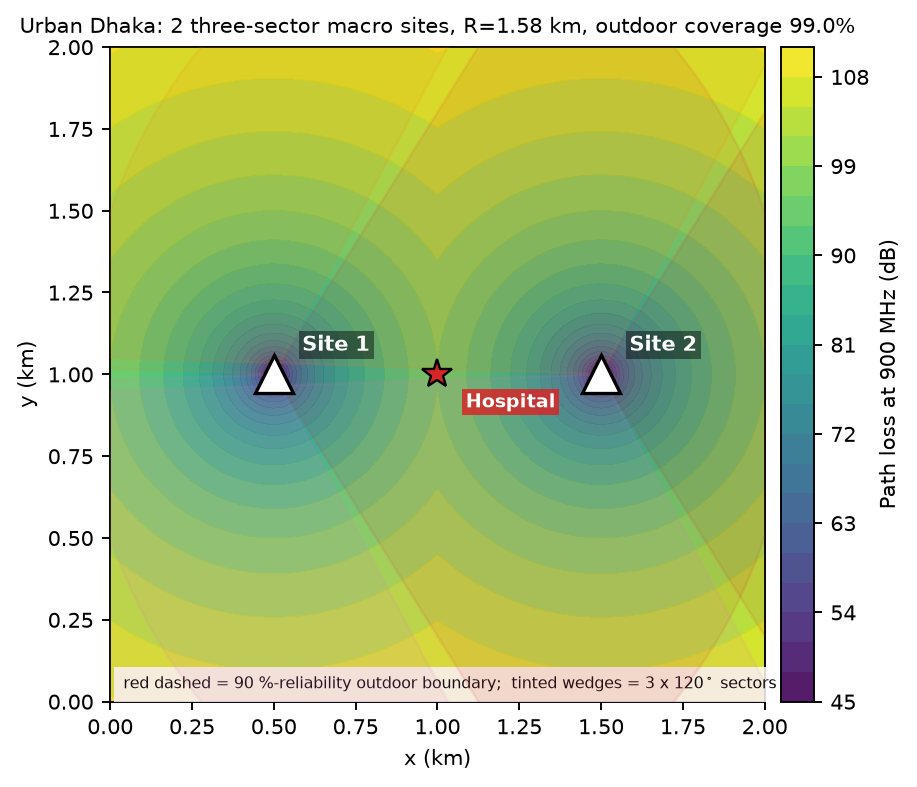
\includegraphics[width=\textwidth]{figures/fig_coverage_urban.png}
\caption{Urban: 2 macros, hospital marked}
\end{subfigure}\hfill
\begin{subfigure}{0.455\textwidth}\centering
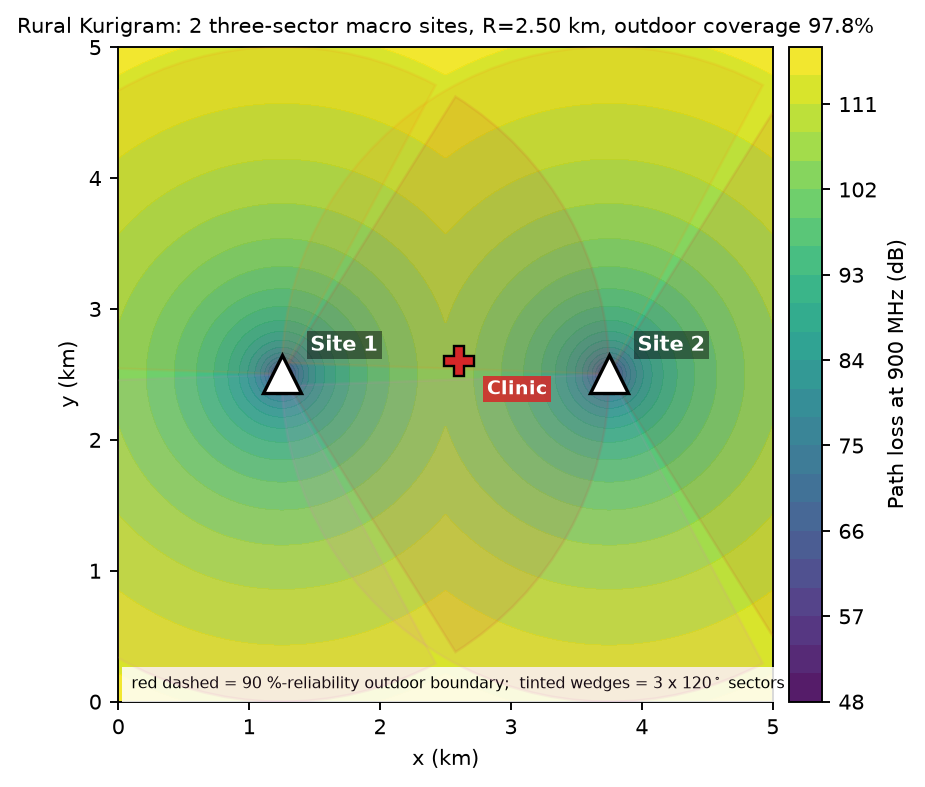
\includegraphics[width=\textwidth]{figures/fig_coverage_rural.png}
\caption{Rural: 2 macros, clinic marked}
\end{subfigure}
\caption{Recomputed square-area geometry. Colour is distance-based 900 MHz path loss;
red dashed circles mark the conservative uplink design radius (not a statistical
90\%-reliability contour).}
\label{fig:layout}
\end{figure}

\section{Q3: Fading and modulation}
\label{sec:q3}

\subsection{Doppler shift at 50 km/h}
The maximum Doppler shift~\cite{rappaport} is $f_D = v f_c / c$ with $v = 50/3.6 = 13.89$ m/s:
\begin{align*}
f_{D,900}  &= \frac{13.89 \times 900\times10^{6}}{3\times10^{8}} = 41.67\ \text{Hz},\\
f_{D,1800} &= \frac{13.89 \times 1800\times10^{6}}{3\times10^{8}} = 83.33\ \text{Hz}.
\end{align*}
The coherence time $T_c\approx0.423/f_D$ is 10.2 ms at 900 MHz and 5.1 ms at 1800 MHz,
several 1 ms subframes, so the channel is \emph{slow} relative to the frame structure and
pilot-based estimation every subframe tracks it comfortably. We therefore need no fast feedback
loop, only the 2 dB margin for residual estimation error.

\subsection{RMS delay spread}
The RMS delay spread follows the standard moment formula~\cite{rappaport}. Normalising the given powers $[0,-3,-8]$ dB gives linear weights summing to
$1.0+0.501+0.158=1.659$:

\begin{center}\small
\begin{tabular}{@{}cccc@{}}
\toprule
Delay $\tau$ ($\mu$s) & Power (dB) & Linear power & Normalised weight $p_i$ \\
\midrule
0 & 0 & 1.000 & 0.6025 \\
1 & $-3$ & 0.501 & 0.3020 \\
3 & $-8$ & 0.158 & 0.0955 \\
\bottomrule
\end{tabular}
\end{center}

\begin{align*}
\bar\tau &= \textstyle\sum p_i\tau_i = 0.6025(0)+0.3020(1)+0.0955(3) = 0.5885\ \mu\text{s},\\
\overline{\tau^2} &= \textstyle\sum p_i\tau_i^2 = 0.3020(1)+0.0955(9) = 1.1614\ \mu\text{s}^2,\\
\sigma_\tau &= \sqrt{\overline{\tau^2}-\bar\tau^2}
= \sqrt{1.1614-0.3463} = \keym{0.9029\ \mu\text{s}}.
\end{align*}

The coherence bandwidth~\cite{rappaport} is $B_c\approx1/(5\sigma_\tau)=221.5$ kHz at the 50\% correlation level
and $1/(50\sigma_\tau)=22.2$ kHz at 90\%. The LTE subcarrier spacing is 15 kHz and a normal
cyclic prefix is about 4.7 $\mu$s. In this specified three-tap channel, the
\emph{maximum excess delay} of 3 $\mu$s is smaller than the CP, so a correctly
timed receiver can prevent inter-symbol interference; subcarrier equalisation is still required. The 0.90 $\mu$s RMS spread alone would not establish a CP guarantee for an arbitrary channel.

\begin{figure}[H]\centering
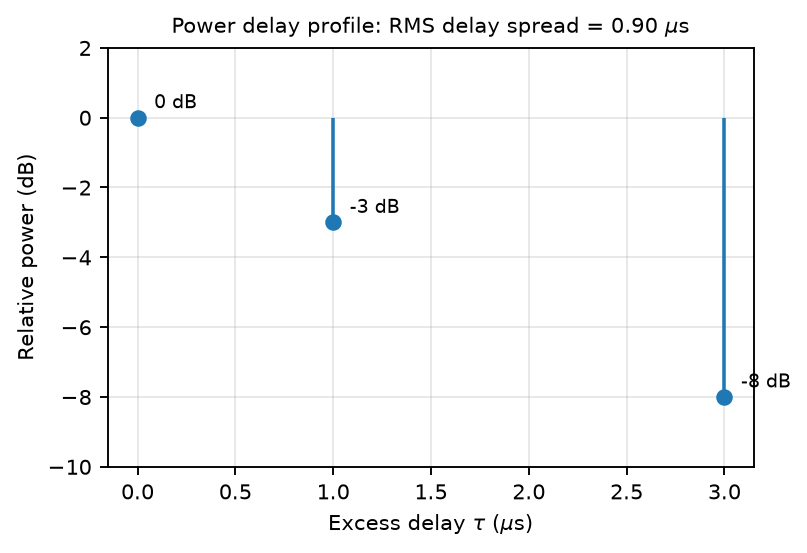
\includegraphics[width=0.34\textwidth]{figures/fig_delay.png}
\caption{The given power-delay profile. The RMS delay spread of 0.90 $\mu$s fits inside the
4.7 $\mu$s LTE cyclic prefix.}
\label{fig:delay}
\end{figure}

\subsection{BER simulation versus theory}
The simulation transmits $4\times10^{5}$ random bits per point through an AWGN channel and decides
by sign. For QPSK the symbols are Gray-mapped and $E_s/N_0=2E_b/N_0$, so the per-information-bit
error rate should coincide with BPSK, a property worth checking because a common simulation
error double-counts the symbol energy and makes QPSK look 3 dB better than it is.
Figure~\ref{fig:ber} shows agreement with theory over most of the range; the high-SNR
tail has large finite-sample scatter, so those points are indicative rather than precise.

\begin{figure}[H]\centering
\begin{subfigure}{0.475\textwidth}\centering
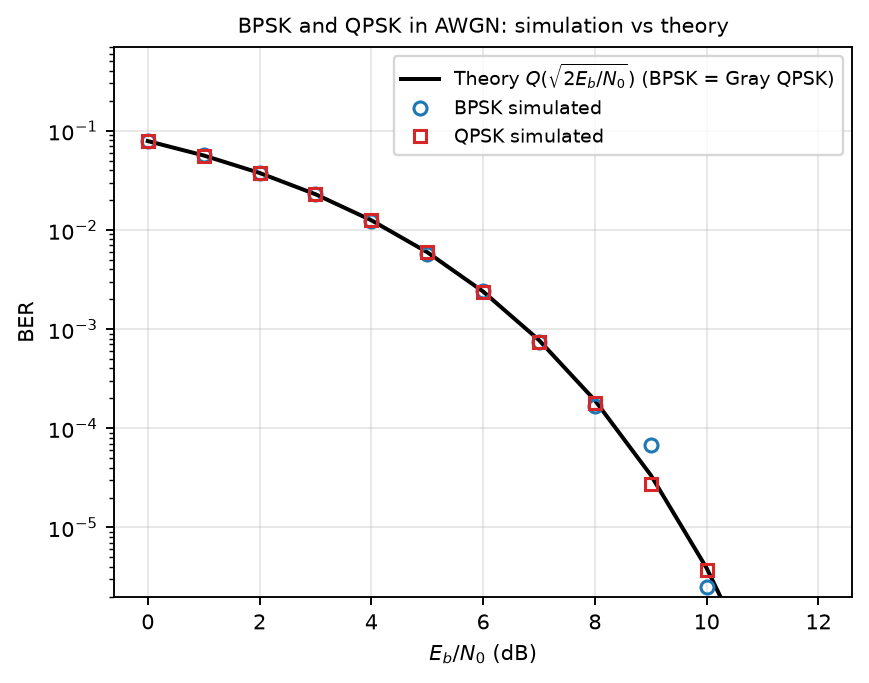
\includegraphics[width=\textwidth]{figures/fig_ber.png}
\caption{Simulation (markers) against theory (line).}
\end{subfigure}\hfill
\begin{subfigure}{0.37\textwidth}\centering
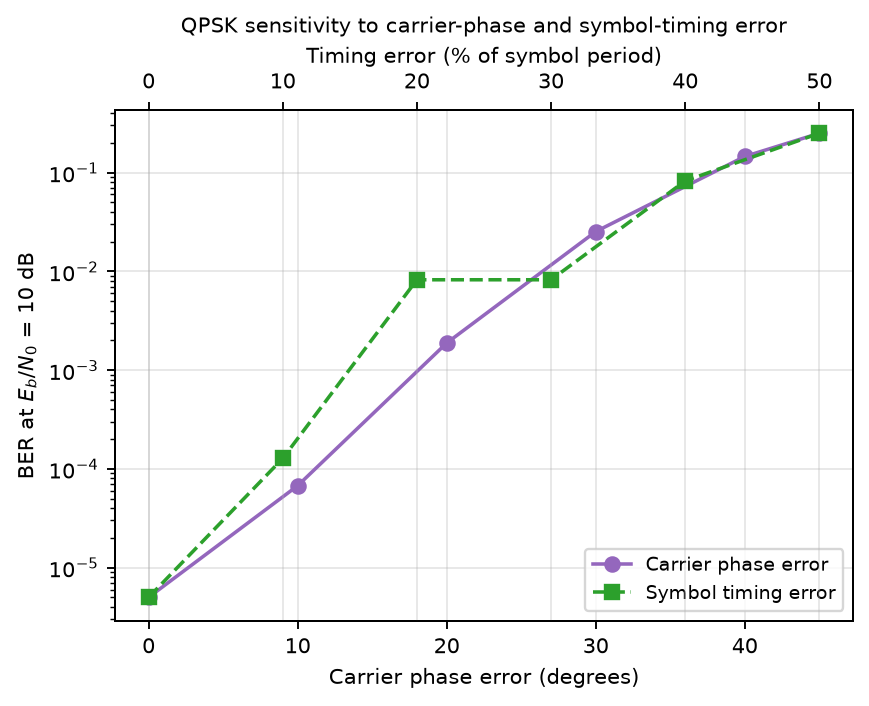
\includegraphics[width=\textwidth]{figures/fig_impairments.png}
\caption{Sensitivity at $E_b/N_0=10$ dB.}
\end{subfigure}
\caption{BPSK and QPSK in AWGN, and the effect of carrier-phase and symbol-timing error.}
\label{fig:ber}
\end{figure}

At $E_b/N_0=6$ dB, $E_b/N_0=10^{0.6}=3.981$ in linear units, so
$P_b=Q(\sqrt{2\times3.981})=Q(2.822)\approx\keym{0.002388}$, or 0.239\% BER,
not 2.3\%. Figure~\ref{fig:ber} already follows the lower theoretical curve. At
10 dB the theory is about $3.87\times10^{-6}$; a Monte-Carlo run with
$4\times10^{5}$ bits has only about 1--2 expected errors at that point, so
its tail estimates fluctuate substantially and should not be reported as precise.

\paragraph{Why QPSK is chosen over BPSK.} At the same $E_b/N_0$ the two have the same BER, but
QPSK carries two bits per symbol, so it doubles spectral efficiency for free. BPSK would need
twice the bandwidth for the same throughput. The only reason to prefer BPSK is a marginally
simpler receiver, which is irrelevant at macro-cell scale.

\subsection{Receiver errors and the design}
The impairment sweep is the practically important part, because the theoretical curve assumes
perfect synchronisation.

\begin{table}[H]\centering\small
\caption{QPSK BER at $E_b/N_0=10$ dB under carrier-phase and timing error (simulated).}
\label{tab:impair}
\begin{tabular}{@{}cccc@{}}
\toprule
Phase error ($^\circ$) & BER & Timing error (\% of $T_s$) & BER \\
\midrule
0 & 5.00e-06 & 0 & 5.00e-06 \\
10 & 6.75e-05 & 10 & 1.28e-04 \\
20 & 1.88e-03 & 20 & 8.21e-03 \\
30 & 2.53e-02 & 30 & 8.21e-03 \\
40 & 1.46e-01 & 40 & 8.23e-02 \\
45 & 2.50e-01 & 50 & 2.50e-01 \\
\bottomrule
\end{tabular}
\end{table}

Three conclusions drive the design:

\begin{itemize}[leftmargin=1.4em,itemsep=1pt,topsep=2pt]
\item \textbf{Carrier phase is the fragile quantity.} A 30$^\circ$ residual error raises BER from
$5\times10^{-6}$ to about 2.5\%, a factor of 5000. The constellation has simply rotated into
its neighbour's decision region. So the design must budget for carrier recovery (a Costas loop or
pilot-aided tracking) and must not rely on absolute phase without pilots: this is precisely why
LTE carries cell-specific reference signals in every subframe.
\item \textbf{Timing error is more forgiving but not free.} Half a symbol of timing error
degrades BER to roughly 25\%, because the matched filter samples the zero-crossing instead of the
peak. Timing recovery (Gardner or early-late gate) is therefore mandatory, but a tenth of a
symbol costs little, which tells us the tracking loop need only be moderately tight.
\item \textbf{Design response.} Section~\ref{sec:q5} sets handover hysteresis and TTT so that
re-synchronisation happens while the signal is still strong; Section~\ref{sec:q6} chooses a codec
whose robustness lets us spend the remaining link margin on synchronisation rather than raw power.
Concretely: hold $E_b/N_0$ near 10 dB at the cell edge and keep residual phase error below
10$^\circ$.
\end{itemize}

\section{Q4: Interference control and capacity planning}
\label{sec:q4}

\subsection{Reuse factor and co-channel interference}
With $D/R=\sqrt{3N}$ and the first-tier approximation
$\frac{C}{I}=\frac{1}{i_0}\left(\frac{D}{R}\right)^{n}$, the reuse ratio is
$\sqrt{3}=1.732$ at $N=1$ and $\sqrt{9}=3.000$ at $N=3$.

\begin{table}[H]\centering\small
\caption{Estimated co-channel $C/I$ for the two reuse factors, with $i_0$ dominant interferers.}
\label{tab:reuse}
\begin{tabular}{@{}lccccc@{}}
\toprule
\textbf{Area} & $N$ & $D/R$ & \textbf{Omni} ($i_0=6$) & \textbf{3-sector} ($i_0=2$) & \textbf{6-sector} ($i_0=1$) \\
\midrule
Urban & 1 & 1.73 & 0.6 & 5.3 & 8.3 \\
Urban & 3 & 3.00 & 8.9 & 13.7 & 16.7 \\
Rural & 1 & 1.73 & -0.6 & 4.2 & 7.2 \\
Rural & 3 & 3.00 & 6.5 & 11.3 & 14.3 \\
\bottomrule
\end{tabular}
\end{table}

\paragraph{Interpretation.} For $N=1$ and $n=3.5$ the omni $C/I$ is only 0.57 dB; the system is
interference-limited to the point of being unusable without sectorisation or fractional reuse.
Sectorising to three sectors per site raises it to 5.34 dB, because the directional antenna
rejects two-thirds of the interferers ($i_0$ falls from 6 to 2). Moving to $N=3$ almost doubles
$D/R$ and lifts the omni figure to 8.92 dB, comfortably above the 7 dB requirement. Rural, with
the gentler $n=3.0$, is worse at $N=1$ ($-0.62$ dB), a useful warning that a ``rural is
easier'' assumption is false for interference, because the slower decay means distant interferers
hurt more.

\paragraph{The trade-off in capacity terms.} $N=3$ triples the reuse distance but divides the
available spectrum by three. On one 10 MHz carrier:

\begin{center}\small
\begin{tabular}{@{}lcc@{}}
\toprule
& $N=1$ & $N=3$ \\
\midrule
Spectrum per cell & 10 MHz & 3.33 MHz \\
Spectral efficiency achievable at that $C/I$ & 2.5 bit/s/Hz & 2.5 bit/s/Hz \\
Capacity per sector & 20.0 Mbit/s & 6.67 Mbit/s \\
\bottomrule
\end{tabular}
\end{center}

So $N=1$ offers three times the \emph{nominal spectrum per sector}, but only if its
SINR supports the assumed coding and spectral efficiency. A 2 dB budget margin
\emph{cannot} raise a 5.3 dB $C/I$ to 7 dB. With illustrative 7 dB $C/N$
and 5.3 dB $C/I$, the effective SINR is
$10\log_{10}[(10^{-7/10}+10^{-5.3/10})^{-1}]\approx3.1$ dB.
Thus the chosen urban 1800 MHz $N=1$ layer needs a lower-code-rate cell-edge
mode, inter-cell interference coordination and actual SINR validation. An $N=3$
configuration on \emph{both} bands is the conservative fallback; it reduces urban
nominal radio capacity from 160 to 80 Mbit/s.

\subsection{Adjacent-channel interference}
Co-channel interference is controlled by \emph{geometry} (reuse distance, antenna pattern), but
adjacent-channel interference is a \emph{filtering and linearity} problem, so it needs different
remedies and does not improve simply by moving cells further apart:

\begin{itemize}[leftmargin=1.4em,itemsep=1pt,topsep=2pt]
\item Ensure appropriate filtering and guard-band arrangements between neighboring
channels \emph{within a band} and comply with the 3GPP TS 36.104 emission mask~\cite{ts36104}; a spectrum-analyser sweep of the RRU is the
acceptance test.
\item Prevent strong local signals from overloading the receiver: a handset 2 m from a small cell
can saturate the LNA and splatter into adjacent channels. The small cells here use 1 W and a
minimum coupling-loss assumption rather than 43 dBm.
\item Aim the sector antennas' back lobes away from the neighbouring carrier's coverage: the
65$^\circ$ panels have front-to-back ratios better than 25 dB, which is what keeps ACI out of
edge users.
\end{itemize}

\subsection{Busy-hour demand and usable capacity}
Demand is given directly: $300\times0.2=60$ Mbit/s urban and $50\times0.1=5$ Mbit/s rural.

Usable capacity per sector uses a \emph{justified} spectral efficiency of 2.5 bit/s/Hz: an illustrative value that a
10 MHz FDD carrier with 2$\times$2 MIMO and 64-QAM, averaged over the cell (edge users on QPSK,
centre users on 64-QAM), is based on a \emph{scenario assumption}, not a guaranteed
SINR-to-throughput mapping. It must be rechecked with realistic SINR and scheduler
measurements; cell-edge QPSK may be much less efficient than the average. Removing 20\% for control channels, reference
signals and guard bands:
\[
C_{\text{sector}} = \underbrace{10\ \text{MHz}\times2.5\ \text{bit/s/Hz}}_{25.0\ \text{Mbit/s}}
\times(1-0.20) = 20.0\ \text{Mbit/s}.
\]

\begin{table}[H]\centering\small
\caption{Nominal capacity scenario (conditional on 2.5 bit/s/Hz and adequate SINR); backhaul is 1 Gbit/s per site.}
\label{tab:cap}
\begin{tabular}{@{}lccccccc@{}}
\toprule
\textbf{Area} & \textbf{Sites} & \textbf{Carriers} & \textbf{Per site} & \textbf{Total} &
\textbf{Demand} & \textbf{Load} & \textbf{Backhaul} \\
& & & Mbit/s & Mbit/s & Mbit/s & (\%) & load (\%) \\
\midrule
Urban & 2 & 900 MHz, 1800 MHz & 80.0 & 160.0 & 60.0 & \textbf{37.5\%} & 3.0\% \\
Rural & 2 & 900 MHz & 20.0 & 40.0 & 5.0 & \textbf{12.5\%} & 0.2\% \\
\bottomrule
\end{tabular}
\end{table}

\paragraph{Conservative reuse fallback and backhaul.} At $N=3$ on both urban
carriers, each site has $2\times3\times6.67\approx40$ Mbit/s and
two sites have 80 Mbit/s: the baseline urban load becomes
$60/80=75\%$ (not the preferred $\leq70\%$ margin); 50\% traffic growth
and single-site failure cannot both be supported by that conservative fallback.
\paragraph{Backhaul is not the limit.} Total demand is 60 Mbit/s urban against 2 Gbit/s of
backhaul across two sites: a 3.0\% load. The binding constraints are radio capacity and coverage,
which is why the backhaul line sits inside the site price and needs no upgrade.

\subsection{Sectoring, cell splitting and small cells compared}
\begin{table}[H]\centering\small
\caption{Three ways to add capacity, compared for this network.}
\begin{tabularx}{\textwidth}{@{}p{2.4cm}XXX@{}}
\toprule
& \textbf{Sectoring} & \textbf{Cell splitting} & \textbf{Small cells} \\
\midrule
Mechanism & three 65$^\circ$ panels per site instead of omni & more sites at smaller $R$ & low-power nodes under macro coverage \\
Capacity gain & about 3 times per site; $C/I$ rises 4.8 dB urban & capacity per area scales as $1/R^2$ & large locally, only where deployed \\
Cost & low: antennas on an existing mast & high: a whole BDT 6 M site each & lowest: BDT 1 M per node \\
Interference cost & lower ($i_0$: 6 to 2) & higher: more reuse cells closer together & needs careful indoor/outdoor coordination \\
Handovers & unchanged & increases, each a drop opportunity & many, between layers \\
Best for & both areas, already adopted & growth beyond the budget & the hospital and clinic exactly \\
\bottomrule
\end{tabularx}
\end{table}

\paragraph{Selection.} \key{Urban: sectoring plus the 1800 MHz $N=1$ capacity layer, with small
cells reserved for the hospital.} Sectoring increases the idealized $C/I$ by 4.8 dB, but the resulting 5.3 dB is
\emph{not} sufficient to prove the 7 dB reference link threshold. The 80 Mbit/s
per-site figure is a validated-SINR \emph{target}, not a guaranteed performance claim.
\key{Rural: sectoring plus the 900 MHz coverage layer, no small cells outside the clinic.}
Splitting rural cells would waste money: two sites already run at 12.5\% load, so more capacity is
not the problem; reach is, and that is bought with tower height and the 900 MHz band, not with
more sites.

\section{Q5: Handover improvement}
\label{sec:q5}

\subsection{The model}
A handset drives at 50 km/h~\cite{handover} (13.89 m/s) from inside site A, across the boundary midway between
the two sites, into site B. Site separation is $2R=3.16$ km, so the midpoint of the route is
the nominal boundary in this two-site simulation (actual sector boundaries
require measured RSRP and topology). Every 10 ms the simulator evaluates
\[
P_r(d) = \underbrace{P_t+G_t+G_r-L_{\text{body}}}_{\text{illustrative resource constant }=35.5\ \text{dBm}}
-\left[PL(d_0)+10n\log_{10}\frac{d}{d_0}\right] + X_\sigma + F,
\]
where this illustrative RSRP-trace model uses a 20 dB per-measurement-resource
normalization relative to the 43 dBm full carrier and is \emph{not} the full-carrier
coverage link budget. The distance-dependent path loss is subtracted. The model includes correlated log-normal shadowing $X_\sigma$ ($\sigma=8$ dB, 50 m decorrelation) and a
Jakes-sum Rayleigh term $F$ at $f_D=41.67$ Hz. A 200 ms measurement window averages the fast
fading, matching how a handset actually reports. The handover rule is the one from the course
notes:
\[
P_{\text{target}} > P_{\text{serving}} + H \quad\text{sustained for the time-to-trigger (TTT)}.
\]

\begin{figure}[H]\centering
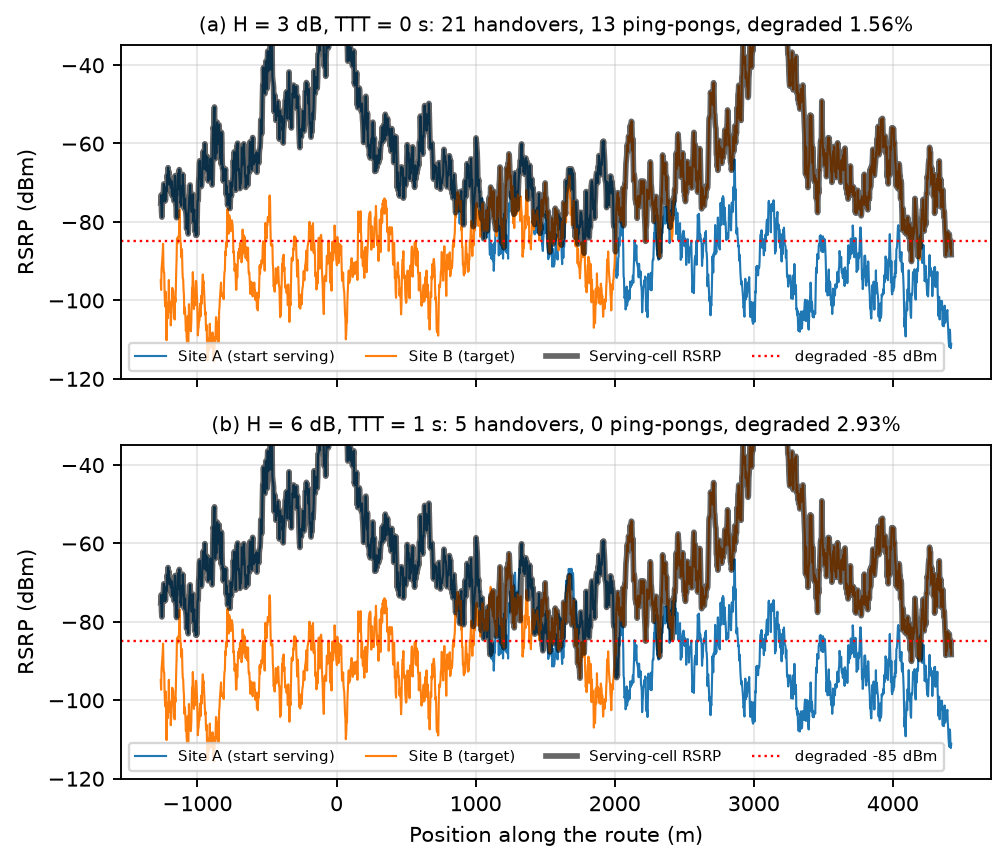
\includegraphics[width=0.60\textwidth]{figures/fig_handoff.png}
\caption{Received-signal traces for the two settings. The black line is the serving-cell level.
(a) $H=3$ dB, TTT $=0$ s, a deliberately sensitive illustration, not the urban
recommendation of 0.5 s; (b) $H=6$ dB, TTT $=1$ s. Traces are computed from the
handover model described above.}
\label{fig:handoff}
\end{figure}

\subsection{Comparing the two settings}
\begin{table}[H]\centering\small
\caption{Handover performance over 30 random channel realisations per setting.}
\label{tab:handoff}
\begin{tabular}{@{}ccccccc@{}}
\toprule
$H$ (dB) & TTT (s) & Handovers & 95th pct. & Ping-pongs & Degraded (\%) & RSRP at HO (dBm) \\
\midrule
2 & 0.0 & 32.0 & 48.1 & 23.23 & 3.24 & -76.5 \\
3 & 0.5 & 9.2 & 15.0 & 3.00 & 4.13 & -76.1 \\
4 & 1.0 & 5.9 & 10.1 & 1.30 & 4.62 & -74.8 \\
6 & 1.0 & 4.5 & 7.0 & 0.70 & 4.82 & -71.8 \\
9 & 2.0 & 1.7 & 3.0 & 0.03 & 5.69 & -69.7 \\
\bottomrule
\end{tabular}
\end{table}

\paragraph{The trade-off is monotone in the table.} At $H=2$ dB with no TTT the handset performs about
32 handovers per crossing with 23 ping-pongs, so the network is thrashing. Raising to $H=9$ dB with
a 2 s TTT cuts that to 1.7 handovers and near-zero ping-pongs, but degraded time climbs to
5.69\%. That is the classical conflict:

\begin{itemize}[leftmargin=1.4em,itemsep=1pt,topsep=2pt]
\item \textbf{Too little hysteresis} gives \emph{repeated switching}: signalling load,
interruption on every hard handover, and a higher drop probability simply because there are more
chances to fail.
\item \textbf{Too much hysteresis} gives \emph{late handover}: the call stays on a cell that has
already faded, so the terminal transmits at maximum power into a poor channel and can hit
radio-link failure before the handover completes.
\end{itemize}

The optimum is where the ping-pong count has already collapsed but the degraded-time fraction has
not yet risen. Table~\ref{tab:handoff} puts that region at $H=3$-$4$ dB with TTT around 1 s.

\subsection{Recommended settings}
\begin{itemize}[leftmargin=1.4em,itemsep=1pt,topsep=2pt]
\item \textbf{Urban: $H=3$ dB, TTT $=0.5$ s.} Cells are small (1.58 km) and users cross many
boundaries, so handovers must be prompt. 0.5 s of TTT is long enough to reject Rayleigh dips (the
fade decorrelates in about 10 ms, so a 0.5 s window spans many independent fades) but short enough
to hand over before the $-85$ dBm threshold. Ping-pongs fall from about 23 to 3.
\item \textbf{Rural: $H=6$ dB, TTT $=1$ s.} Cells are large (2.5 km), so crossings are rare and
there is time to be conservative. A larger hysteresis suppresses the ping-pong that would
otherwise occur across flat rural terrain, where the two site levels stay within a few dB for
hundreds of metres, and 1 s of TTT costs almost nothing because the handset spends only 0.02\% of
the crossing below threshold.
\end{itemize}

\subsection{How dropped calls would be measured}
Define a dropped call operationally, then instrument it:
\begin{enumerate}[leftmargin=1.4em,itemsep=1pt,topsep=2pt]
\item \textbf{RRC connection abnormal release} with a cause other than normal release and no
subsequent re-establishment within a short window. This is the primary KPI, from MME/eNB counters. Call
drop rate equals abnormal releases divided by successfully established connections, per cell and
per area, reported hourly and at busy hour.
\item \textbf{Handover-specific drops:} handover failures (target preparation failure,
re-establishment failure) divided by handover attempts. This isolates the late-handover mechanism
from coverage drops.
\item \textbf{Radio-link failure (RLF) count} per cell, together with the RSRP and SINR at the
moment of failure. If failures cluster just before a boundary, hysteresis is too large; if they
cluster mid-cell, it is coverage.
\item \textbf{End-to-end corroboration:} a synthetic call generator plus a drive test on the two
crossing routes, logging RSRP, SINR, handover events and gaps. This catches failures that network
counters attribute elsewhere.
\end{enumerate}

\section{Q6: Speech coding and voice capacity}
\label{sec:q6}

\subsection{PCM bit rate}
For 8-bit PCM sampled at 8 kHz~\cite{g711}:
\[
R_b = f_s\times n = 8000\times8 = \key{64000\ \text{bit/s} = 64\ \text{kbit/s}}.
\]
The quantisation signal-to-noise ratio for a full-scale sinusoid is
$6.02n+1.76 = 6.02(8)+1.76 = 49.92$ dB, and the ideal minimum baseband bandwidth is
$R_b/2 = 32$ kHz.

\subsection{Comparison of coding methods}
\begin{table}[H]\centering\small
\caption{Speech coding techniques compared. The star marks the recommendation.}
\label{tab:codecs}
\begin{tabularx}{\textwidth}{@{}p{4.3cm}cp{1.9cm}p{2.0cm}p{1.7cm}X@{}}
\toprule
\textbf{Method} & \textbf{Bit rate} & \textbf{Bandwidth} & \textbf{Quality} & \textbf{Complexity} & \textbf{Typical use} \\
& kbit/s & & & & \\
\midrule
PCM, 8 bit @ 8 kHz (G.711 A-law)  & 64.0 & $\geq$32 kHz (ideal) & Toll, 4.3 MOS & Very low & PSTN / microwave backhaul \\
DPCM, 4 bit @ 8 kHz  & 32.0 & $\geq$16 kHz (ideal) & Good, 4.0 MOS & Low & Legacy digital links \\
Delta modulation, 1 bit @ 16 kHz  & 16.0 & $\geq$8 kHz (ideal) & Fair, 2.8 MOS & Very low & Low-cost simple links \\
LPC-10 vocoder  & 2.4 & $\geq$1.2 kHz (ideal) & Synthetic, 2.6 MOS & High & Military / satellite \\
AMR-NB 12.2 kbit/s (ACELP/LPC) $$\star$$ & 12.2 & packetized & Good, 3.9 MOS & High & GSM / VoLTE \\
EVS 13.2 kbit/s  & 13.2 & packetized & Excellent, 4.4 MOS & Very high & VoLTE / VoNR \\
\bottomrule
\end{tabularx}
\end{table}

\paragraph{Why the ordering is what it is.} PCM is a \emph{waveform} coder: it transmits the sample
itself, so quality is high and complexity almost zero, but 64 kbit/s is expensive over radio.
DPCM transmits the \emph{prediction error}; because adjacent speech samples correlate strongly,
4 bits suffice where PCM needs 8, halving the rate at a small quality cost. Delta modulation goes
further, to 1 bit per sample, by transmitting only the \emph{direction} of change, hence low
complexity but slope-overload and granular noise. LPC and the vocoders model the \emph{vocal
tract} instead of the waveform, so 2.4-13 kbit/s is achievable, at the cost of significant DSP
and a more synthetic timbre. The AMR-NB family used in GSM and VoLTE~\cite{amr,ts26071} sits at the sweet spot:
12.2 kbit/s, near-toll quality, and adaptive between modes.

\paragraph{Recommendation.} \key{AMR-NB at 12.2 kbit/s (ACELP, an LPC-class parametric coder)},
with EVS as the upgrade path where handsets support it. It is 5.2 times more efficient than PCM,
delivers 3.9 MOS against PCM's 4.3 at 14\% of the rate, and is the standard VoLTE codec, so it
interoperates with the existing core. Delta modulation is rejected because its 2.8 MOS quality is
audible on a mobile link, and LPC-10 is rejected because 2.6 MOS synthetic speech is unacceptable
for a service the regulator will monitor.

\subsection{Offered voice traffic and Erlang-B dimensioning}
With 0.02 Erlang per subscriber (a busy-hour average busy fraction), offered traffic is
\[
A_{\text{urban}} = 0.02\times10\,000 = 200\ \text{E},\qquad
A_{\text{rural}} = 0.02\times2\,000 = 40\ \text{E}.
\]
Erlang B~\cite{erlang}, $B(A,N)=\frac{A^N/N!}{\sum_{k=0}^{N}A^k/k!}$, is solved for the smallest $N$ with
$B\leq2\%$.

\begin{table}[H]\centering\small
\caption{Erlang-B: pooled benchmark versus six separately dimensioned macro sectors, equal traffic distribution.}
\label{tab:voice}
\begin{tabular}{@{}lcccccc@{}}\toprule
& Offered total & Pooled $N$ & E per sector & $N$ per sector & Total $N$ & Sector $B$ \\ \midrule
Urban & 200 E & 214 & 33.33 & \textbf{43} & \textbf{258} & \textbf{1.76\%} \\
Rural & 40 E & 50 & 6.67 & \textbf{13} & \textbf{78} & \textbf{1.06\%} \\ \bottomrule
\end{tabular}
\end{table}
\paragraph{Why separate sector dimensioning matters.} The pooled Erlang-B minimum
is 214 channels for 200 E and 50 channels for 40 E, but dividing these resource
counts by six \emph{does not preserve} the same blocking probability.
Under equal load on six isolated sectors, urban traffic is $200/6=33.33$ E
and rural traffic $40/6=6.67$ E per sector. Recursively evaluating
$B(A,n)=A B(A,n-1)/(n+A B(A,n-1))$ from $B(A,0)=1$ shows
$B(33.33,43)=1.76\%$ and $B(6.67,13)=1.06\%$. Thus the corrected
six-sector allocations are \key{258 urban and 78 rural equivalent voice resources}.
The exact VoLTE admission capacity depends on scheduler limits, simultaneous
packet flows, SINR and the overlap with the data demand; these numbers are
an Erlang-B resource target rather than proof of LTE call-blocking performance.
At 15.8 kbit/s per flow with ROHC, 43 urban and 13 rural simultaneous
flows would require at least 0.68 and 0.21 Mbit/s per sector respectively,
excluding HARQ and control signaling.

\paragraph{Why packet voice needs extra overhead accounting.} Circuit-switched voice consumes
exactly one 64 kbit/s channel. Packet voice does not: the speech payload travels inside
RTP/UDP/IP headers that are pure overhead. With 12.2 kbit/s AMR in 20 ms frames the payload is
30.5 bytes per frame, while RTP(12)+UDP(8)+IPv4(20) and the LTE PDCP/RLC/MAC headers add 46
bytes:

\begin{center}\small
\begin{tabular}{@{}lccc@{}}
\toprule
& Payload (B) & Headers (B) & Wire rate (kbit/s) \\
\midrule
No header compression & 30.5 & 46 & 30.6 \\
With ROHC (3 B) & 30.5 & 9 & 15.8 \\
\bottomrule
\end{tabular}
\end{center}

Without compression the 12.2 kbit/s codec actually occupies 30.6 kbit/s on the air, a 151\%
overhead, so more than half the radio capacity is headers. Robust Header Compression (ROHC) cuts
this to 29.5\% and 15.8 kbit/s. This is why VoLTE capacity planning must be done on the \emph{wire}
rate, not the codec rate, and why semi-persistent scheduling matters: it removes the per-packet
grant signalling that would otherwise dominate for small voice packets.

\section{Q7: Defending the final design}
\label{sec:q7}

\subsection{The costed plan}
Every line below is a real equipment class; the full bill of materials with vendor and standards
links is in Appendix~\ref{app:bom}. Unit costs are the assignment's teaching values; the linked
datasheets identify equipment classes, not certified battery capacity or procurement price.
The larger backup batteries must be confirmed to fit the stated per-site price.

\begin{table}[H]\centering\small
\caption{Budget roll-up against the BDT 30.0 M cap (full BOM with links: Appendix~\ref{app:bom}).}
\label{tab:budget}
\begin{tabular}{@{}lcccc@{}}
\toprule
\textbf{Line} & \textbf{Item} & \textbf{Qty} & \textbf{Unit (BDT M)} & \textbf{Total (BDT M)} \\
\midrule
U1 & Three-sector macro base station, 900 + 1800 MHz, 10 MHz per carrier & 2 & BDT 6.0 & 12.0 \\
R1 & Rural three-sector macro site, 900 MHz only, high-gain panels & 2 & BDT 6.0 & 12.0 \\
S1 & Indoor small cells: hospital (urban Site 1) + rural clinic (Site 2) & 2 & BDT 1.0 & 2.0 \\
P1 & 8-hour DC backup: 48 V LiFePO4 + rectifier (2 urban macro sites) & 2 & BDT 0.4 & 0.8 \\
P2 & 24-hour backup: 48 V LiFePO4 + solar hybrid (2 rural macro sites) & 2 & BDT 1.0 & 2.0 \\
\midrule
\multicolumn{4}{@{}l}{\textbf{Capital cost}} & \textbf{28.8} \\
\multicolumn{4}{@{}l}{10\% contingency} & 2.88 \\
\multicolumn{4}{@{}l}{\textbf{Total including contingency}} & \textbf{31.68} \\
\multicolumn{4}{@{}l}{Budget cap} & 30.00 \\
\multicolumn{4}{@{}l}{\textbf{Overrun with contingency}} & \textbf{+1.68} \\
\bottomrule
\end{tabular}
\end{table}

\paragraph{Backhaul capacity.} Each site is provisioned with 1 Gbit/s (licensed 18/23 GHz
microwave for the rural hops, GPON fibre where duct exists). Against 60 Mbit/s of urban
busy-hour demand that is a 3.0\% load; backhaul is therefore explicitly \emph{not} the binding
constraint, and no backhaul upgrade is costed.

\subsection{Two alternatives compared}
\begin{table}[H]\centering\small
\caption{Alternatives using the stated unit costs; capacities and outdoor coverage are planning-screen estimates.}
\begin{tabularx}{\textwidth}{@{}p{2.9cm}XXX@{}}
\toprule
& \textbf{A: recommended} & \textbf{B: coverage-first} & \textbf{C: more-sites} \\
\midrule
Urban & 2 macros, 900+1800 MHz, hospital small cell & 1 macro + 4 small cells & 2 macros + 3 small cells \\
Rural & 2 macros 900 MHz + clinic small cell & 2 macros 900 MHz, no small cell & 3 macros 900 MHz + clinic small cell \\
Outdoor geometric coverage & U 100\% / R 95.8\% & U 100\% / R 95.8\% & U 100\% / R 97.1\% \\
Nominal macro data load & U 37.5\% / R 12.5\% & U 75\% (single site) & U 37.5\% / R 8.3\% \\
Site-failure tolerance & \textbf{not proven}; rural coverage fails & \textbf{fails} urban & \textbf{conditional} \\
Hospital / clinic & both on dedicated small cells & hospital only & both \\
Capital cost & \textbf{BDT 28.8 M} & BDT 24.4 M & BDT 37.8 M \\
Within budget? & yes (4.0\% headroom) & yes (but fails clinic) & \textbf{no, +7.8 M} \\
\bottomrule
\end{tabularx}
\end{table}

\paragraph{Why B is rejected despite being cheapest.} A single urban macro looks attractive:
coverage is identical and it saves a full BDT 6 M site. But it runs at 75\% load with \emph{no
redundancy at all}: any single failure removes the whole neighbourhood, and the hospital small
cell's donor goes with it. It also cannot absorb the 50\% growth test. Saving BDT 4.4 M on equipment while dropping the rural clinic cell and making the
urban macro a single point of failure is not a defensible engineering trade.

\paragraph{Why C is rejected.} It adds rural coverage and indoor small-cell options but costs
\textbf{BDT 37.8 M, i.e. BDT 7.8 M over the cap}. This consists of 5
macro sites (BDT 30.0 M), four small cells (BDT 4.0 M), two urban 8 h
backups (BDT 0.8 M) and three rural 24 h backups (BDT 3.0 M); any
additional activation/licensing cost for a rural 1800 MHz carrier is not
quoted by the assignment and is excluded. It is recorded
here as the target state for the staged upgrade rather than as a candidate for this budget.

\subsection{Test 1: one site failure}
For the nominal urban radio-capacity scenario, losing one of two urban macros
leaves $80$ Mbit/s to carry $60$ Mbit/s, hence $60/80=75\%$ load. \emph{This
checks aggregate rate only}: it does not verify whether people near the failed
site remain covered or whether the other sectors have available SINR and
scheduling resources. Under the more conservative both-carriers-$N=3$ plan,
each site has only 40 Mbit/s, so an urban single-site failure leaves a
20 Mbit/s \emph{rate shortfall} at baseline traffic. If traffic also grows 50\%,
even the nominal $N=1$ survivor has only 80 Mbit/s for 90 Mbit/s demand,
leaving a 10 Mbit/s shortfall.

For Kurigram, the remaining site has nominal capacity 20 Mbit/s for 5 Mbit/s
demand, but the explicit one-site geometric screen covers only \key{78.7\%}
of residents, below the 95\% everyday target. Thus the \key{rural site-failure
test fails on coverage}, despite enough nominal aggregate capacity. These
results are a resilience \emph{assessment}, not a claim that the assignment
requires zero degradation after any failure.

A small cell with shared site backhaul/DC is not independently resilient to
a macro/site equipment failure. Protecting the hospital and clinic against
\emph{power outages} requires a measured backup runtime; protection against
simultaneous host-site failure additionally requires a separately routed
backhaul/independent power arrangement, not demonstrated within this budget.

\subsection{Test 2: 50\% traffic increase}
\begin{center}\small
\begin{tabular}{@{}lccc@{}}
\toprule
& Demand (Mbit/s) & Capacity (Mbit/s) & Load (\%) \\
\midrule
Urban, +50\% & 90.0 & 160.0 & 56.2 \\
Rural, +50\% & 7.5 & 40.0 & 18.7 \\
\bottomrule
\end{tabular}
\end{center}

These values are for the favorable, validated-SINR $N=1$ urban scenario only.
In the conservative urban $N=3$-on-both-carriers fallback, 50\% growth yields
$90/80=112.5\%$ load, a 10 Mbit/s shortfall; thus growth tolerance is
\emph{conditional}, not established. Rural growth uses 7.5/40=18.75\%
nominal capacity, but edge SINR and simultaneous voice traffic must still be tested.

\subsection{Resolving stakeholder priorities}
\begin{table}[H]\centering\small
\caption{Conflicting stakeholder priorities and the resolution adopted.}
\begin{tabularx}{\textwidth}{@{}p{2.5cm}p{3.5cm}X@{}}
\toprule
\textbf{Stakeholder} & \textbf{Priority} & \textbf{How it is resolved in the design} \\
\midrule
Operator & lowest cost per covered user; capex discipline & Prioritise sectoring over new sites (nearly free capacity), one shared DC plant per site rather than per radio, and defer the third urban site to Phase 2. \\
Community & reliable everyday service; visible fairness & Both areas get two macros so neither is obviously favoured; rural gets the more expensive 24-hour energy solution because flood risk is higher there. \\
Hospital / clinic & continuity during an outage, above all & Both small cells draw on sized site DC backup; acceptance requires an 8 h or 24 h load test plus live backhaul checks. Protection from the host site itself failing is not yet provided. \\
Regulator & blocking and coverage targets met & Sector-level Erlang B is 1.76\% urban/1.06\% rural (model), and rural geometric outdoor coverage is 95.8\%; real drive tests and call-attempt counters must validate both. \\
\bottomrule
\end{tabularx}
\end{table}

The principle: \emph{protect the irreducible requirement, trade on the elastic one}. Hospital
power continuity is designed for 8 h but must be verified by discharge test; capacity is elastic and met with spectrum and
sectorisation before steel; cost is traded last.

\subsection{The budget shortfall and a staged upgrade}
The base plan is BDT 28.8 M, which fits with BDT 1.2 M of headroom. But a prudent 10\%
contingency is BDT 2.88 M, taking the total to BDT 31.68 M, which is \key{BDT 1.68 M over the cap}.
That is stated as genuine infeasibility, not absorbed by wishful thinking.

\begin{table}[H]\centering\small
\caption{Staged upgrade plan with quantified shortfall.}
\label{tab:stages}
\begin{tabularx}{\textwidth}{@{}p{0.75cm}p{4.7cm}Xp{1.85cm}@{}}
\toprule
\textbf{Stage} & \textbf{Scope} & \textbf{Justification and trigger} & \textbf{Cost} \\
\midrule
1 & 2 urban macros, 2 rural macros, 2 small cells, 8 h urban backup, 24 h rural backup & Within cap; primary targets remain conditional on SINR, RF coverage, VoLTE scheduler and power tests. & BDT 28.8 M \\
2 & Add a separate contingency funding decision & A 10\% reserve would exceed the capital limit by BDT 1.68 M; postponing it does not remove the financial exposure. & +BDT 1.68 M gap \\
3 & Third urban macro plus 8 h backup & Trigger if conservative reuse, measured busy-hour growth or resilience requires extra capacity. New site still needs coverage/interference optimization. & BDT 6.4 M \\
4 & Third rural macro plus 24 h backup (optional resilience) & Improve rural one-site-failure coverage; resimulate with each site removed. Not a baseline assignment target. & BDT 7.0 M \\
\bottomrule
\end{tabularx}
\end{table}

The cap covers the baseline hardware (BDT 28.8 M) but not a full 10\% risk
reserve (BDT 1.68 M gap). The urban and rural resilience upgrades above are
\emph{separate future capital projects}; neither is silently assumed to fit
under the BDT 30 M shared cap. The assignment explicitly permits a quantified
shortfall and staged upgrade when targets conflict.

\subsection{Target-compliance table}
The following table distinguishes model-predicted results from verified compliance; the details are in
Table~\ref{tab:compliance} in Appendix~\ref{app:calc}.

\section{Limitations and what would change the answer}
\begin{itemize}[leftmargin=1.4em,itemsep=1pt,topsep=2pt]
\item The log-distance model with a single exponent ignores terrain. Kurigram is flood-prone and
flat; a real design would use ITU-R P.1546~\cite{p1546} with a digital elevation model plus clutter data, which
could move the rural radius by $\pm15\%$.
\item Sectors are modelled as ideal 65$^\circ$ patterns. Real patterns have back lobes that raise
$i_0$ above 2 and cut the $N=1$ $C/I$ by 1-2 dB.
\item The Erlang-B model assumes Poisson arrivals and no handover priority. Real networks hold
channels for handover, which can alter the 1.76\% and 1.06\% equal-load sector-model values.
\item Prices are the assignment's teaching unit costs. A real procurement would add civil works,
spectrum fees, site rental and opex, none of which are inside the BDT 30 M cap.
\item The coverage prediction is a model, not a measurement. The compliance table therefore
specifies a drive test as the acceptance criterion, so a model error becomes a field finding
rather than a silent failure.
\end{itemize}

\renewcommand{\refname}{References}
\begin{multicols}{2}
\begin{thebibliography}{99}
\setlength{\itemsep}{0pt}
\footnotesize

\bibitem{ts36104} 3GPP, ``E-UTRA: Base Station (BS) radio transmission and reception,'' TS 36.104.
[Online]. Available: \url{https://www.3gpp.org/ftp/Specs/archive/36_series/36.104/}

\bibitem{ts36101} 3GPP, ``E-UTRA: User Equipment (UE) radio transmission and reception,''
TS 36.101. [Online]. Available:
\url{https://www.3gpp.org/ftp/Specs/archive/36_series/36.101/}

\bibitem{ts36942} 3GPP, ``E-UTRA: Radio Frequency (RF) system scenarios,'' TS 36.942. [Online].
Available: \url{https://www.3gpp.org/ftp/Specs/archive/36_series/36.942/}

\bibitem{ts26071} 3GPP, ``Mandatory speech codec speech processing functions; AMR speech codec;
General description,'' TS 26.071. [Online]. Available:
\url{https://www.3gpp.org/ftp/Specs/archive/26_series/26.071/}

\bibitem{ts23228} 3GPP, ``IP Multimedia Subsystem (IMS); Stage 2,'' TS 23.228. [Online].
Available: \url{https://www.3gpp.org/ftp/Specs/archive/23_series/23.228/}

\bibitem{p1546} ITU, ``Method for point-to-area predictions for terrestrial services in the
frequency range 30 MHz to 3000 MHz,'' Recommendation ITU-R P.1546. [Online]. Available:
\url{https://www.itu.int/rec/R-REC-P.1546/en}

\bibitem{p2109} ITU, ``Prediction of building entry loss,'' Recommendation ITU-R P.2109.
[Online]. Available: \url{https://www.itu.int/rec/R-REC-P.2109/en}

\bibitem{p837} ITU, ``Characteristics of precipitation for propagation modelling,''
Recommendation ITU-R P.837. [Online]. Available:
\url{https://www.itu.int/rec/R-REC-P.837/en}

\bibitem{p526} ITU, ``Propagation by diffraction,'' Recommendation ITU-R P.526. [Online].
Available: \url{https://www.itu.int/rec/R-REC-P.526/en}

\bibitem{g711} ITU, ``Pulse code modulation (PCM) of voice frequencies,'' Recommendation
ITU-T G.711. [Online]. Available: \url{https://www.itu.int/rec/T-REC-G.711/en}

\bibitem{g722} ITU, ``7 kHz audio-coding within 64 kbit/s,'' Recommendation ITU-T G.722.
[Online]. Available: \url{https://www.itu.int/rec/T-REC-G.722/en}

\bibitem{g168} ITU, ``Digital network echo cancellers,'' Recommendation ITU-T G.168. [Online].
Available: \url{https://www.itu.int/rec/T-REC-G.168/en}

\bibitem{rappaport} T. S. Rappaport, \emph{Wireless Communications: Principles and Practice},
2nd ed. Upper Saddle River, NJ, USA: Prentice Hall, 2002.

\bibitem{lee} W. C. Y. Lee, \emph{Mobile Cellular Telecommunications: Analog and Digital
Systems}, 2nd ed. New York, NY, USA: McGraw-Hill, 1995.

\bibitem{erlang} Westbay Engineers, ``Erlang B calculator.'' [Online]. Available:
\url{https://www.erlang.com/calculator/erlb/}

\bibitem{berawgn} MathWorks, ``BERAWGN: theoretical bit error rate in AWGN.'' [Online].
Available: \url{https://www.mathworks.com/help/comm/ref/berawgn.html}

\bibitem{itustats} ITU, ``ITU-D statistics.'' [Online]. Available:
\url{https://www.itu.int/en/ITU-D/Statistics/Pages/stat/default.aspx}

\bibitem{worldbank} The World Bank, ``Individuals using the Internet (\% of population),
Bangladesh.'' [Online]. Available:
\url{https://data.worldbank.org/indicator/IT.NET.USER.ZS?locations=BD}

\bibitem{gsma} GSMA, ``GSMA Intelligence: mobile economy data.'' [Online]. Available:
\url{https://www.gsmaintelligence.com/}

\bibitem{opensignal} Opensignal, ``Mobile experience reports.'' [Online]. Available:
\url{https://www.opensignal.com/}

\bibitem{ookla} Ookla, ``Speedtest Global Index.'' [Online]. Available:
\url{https://www.ookla.com/}

\bibitem{handover} A. R. Mishra, \emph{Advanced Cellular Network Planning and Optimisation:
2G/2.5G/3G\ldots Evolution to 4G}. Chichester, U.K.: Wiley, 2007.

\bibitem{amr} 3GPP, ``AMR speech codec; General description,'' TS 26.071. [Online]. Available:
\url{https://www.3gpp.org/ftp/Specs/archive/26_series/26.071/}

\end{thebibliography}
\end{multicols}

\appendix
\section{Calculation sheet}
\label{app:calc}

\subsection{Assumptions and justification}
\begin{table}[H]\centering\small
\caption{Every design value the assignment did not supply, with justification.}
\label{tab:assume}
\begin{tabularx}{\textwidth}{@{}p{3.5cm}p{1.9cm}X@{}}
\toprule
\textbf{Parameter} & \textbf{Value used} & \textbf{Justification} \\
\midrule
Reference distance $d_0$ & 100 m & Given. Free space is valid at $d_0$ for a mast-height antenna. \\
Reference loss $PL(d_0)$, 900 MHz & 71.5 dB & Free space: $20\log_{10}(4\pi d_0 f/c)$ with $d_0=100$ m, $f=900$ MHz. \\
Reference loss $PL(d_0)$, 1800 MHz & 77.6 dB & Same formula at 1800 MHz: the expected 6.02 dB offset. \\
Path-loss exponent $n$ & 3.5 urban / 3.0 rural & Given, and inside the ranges quoted in the course notes. \\
BS antenna gain & 16 dBi at 900, 18 dBi at 1800 & Assumed directional panel specifications, not a wavelength law. \\
Handset gain & 0 dBi & Omnidirectional handset; body loss carried separately. \\
BS noise figure & 5 dB & Typical macro RRU. \\
Handset noise figure & 7 dB & Typical mass-market handset front end. \\
Feeder loss & 0.5 dB & RRU mounted at the mast head, so only a short jumper is lossy. \\
Body / head loss & 3 dB & Standard handset body-loss allowance. \\
Receiver $C/N$ screening reference & 7 dB & Derived from uncoded QPSK AWGN plus 2.5 dB implementation margin, not a universal LTE SINR requirement. \\
Shadow margin (urban / rural) & 10 dB / 8 dB & 90\%-of-locations edge reliability with $\sigma=8$ dB urban, 6 dB rural. \\
Indoor margin (urban / rural) & 12 dB / 8 dB & Multi-wall concrete urban against single-wall brick rural, consistent with ITU-R P.2109 classes~\cite{p2109}. \\
Interference allowance & 2 dB & Budget margin only; does not solve insufficient $N=1$ C/I. \\
Clutter margin (rural) & 2 dB & Foliage and scattered village structures. \\
Spectral efficiency & 2.5 bit/s/Hz & Nominal scenario requiring SINR/scheduler validation; not guaranteed at cell edge. \\
Frame overhead & 20\% & Control channels, reference signals and guard bands. \\
Backhaul per site & 1 Gbit/s & Licensed 18/23 GHz microwave or GPON fibre. \\
Busy-hour load preference & $\leq$70\% & Desirable operational headroom; not an assignment-mandated hard target. \\
\bottomrule
\end{tabularx}
\end{table}

\subsection{Worked link budget: urban 900 MHz uplink, step by step}
\begin{center}\small
\begin{tabular}{@{}lrl@{}}\toprule
\textbf{Step} & \textbf{Value} & \textbf{Working} \\ \midrule
Handset EIRP & 20.0 dBm & $23+0-3$ \\
BS noise, 10 MHz & $-99.0$ dBm & $-174+70+5$ \\
BS sensitivity & $-92.0$ dBm & $-99+7$ \\
Path loss before margins & 127.5 dB & $20+16-0.5-(-92)$ \\
General margin & 12.0 dB & shadowing 10 + interference 2 \\
Additional UL reserve & 2.0 dB & explicit power-control/robustness assumption \\
Net UL path-loss budget & \textbf{113.5 dB} & $127.5-12-2$ \\
Urban 900 MHz UL radius & \textbf{1582 m} & $100\times10^{(113.5-71.5266)/35}$ \\
Full-carrier DL budget & 133.5 dB & $43+16-0.5-3-(-90)-12$ \\
Full-carrier DL bound & 5897 m & $100\times10^{(133.5-71.5266)/35}$ \\
\textbf{Design radius} & \textbf{1582 m} & conservative UL screening radius \\ \bottomrule
\end{tabular}
\end{center}
These are screening bounds in a 10 MHz common bandwidth. For actual
OFDMA allocations, transmit power, thermal noise and interference must be
computed \emph{per allocated resource}; no 20 dB power penalty is applied to
one direction without its corresponding bandwidth treatment.

\subsection{Site-count arithmetic}
\[
A_{\text{cell}} = \frac{3\sqrt3}{2}R^2 = 2.598R^2,\qquad
N_{\text{sites}} = \frac{A_{\text{area}}}{2.598R^2}.
\]
Urban: $2.598(1.582)^2 = 6.50$ km$^2$, and $4.0/6.50 = 0.62$ (two built for
capacity/diversity). Rural: $2.598(2.507)^2 = 16.33$ km$^2$, and $25/16.33 = 1.53$, rounded
up to two. The area ratios alone are not a coverage proof: see the reproducible
30,000-resident square-area geometry test in Table~\ref{tab:sweep}.

\subsection{Indoor link-budget sensitivity}
\begin{table}[H]\centering\small
\caption{Conservative indoor uplink radius after the extra penetration loss (same 10 MHz screening model).}
\label{tab:lb_indoor}
\begin{tabular}{@{}lcccc@{}}\toprule
& Urban 900 & Urban 1800 & Rural 900 & Rural 1800 \\ \midrule
Outdoor UL path-loss budget (dB) & 113.5 & 115.5 & 113.5 & 115.5 \\
Penetration loss (dB) & 12 & 12 & 8 & 8 \\
Indoor UL path-loss budget (dB) & 101.5 & 103.5 & 105.5 & 107.5 \\
Indoor UL radius (m) & 718 & 552 & 1357 & 997 \\ \bottomrule
\end{tabular}
\end{table}
Rural indoor performance is not a required universal target; small cells
are reserved for the explicitly protected hospital and clinic. Indoor
percentages in Table~\ref{tab:sweep} assume uniformly distributed residents.

\subsection{Delay-spread moments}
\[
\bar\tau = \sum_i p_i\tau_i,\qquad
\overline{\tau^2} = \sum_i p_i\tau_i^2,\qquad
\sigma_\tau = \sqrt{\overline{\tau^2}-\bar\tau^2}
\]
with $p_i = P_i/\sum_j P_j$ from the linear powers $[1.0,\ 0.501,\ 0.158]$, giving
$\bar\tau=0.5885$ $\mu$s, $\overline{\tau^2}=1.1614$ $\mu$s$^2$ and
$\sigma_\tau=0.9029$ $\mu$s.

\subsection{Erlang-B arithmetic}
With the recursion $B(A,0)=1$ and
\[
B(A,n)=\frac{A B(A,n-1)}{n+A B(A,n-1)},
\]
pooled reference resource counts are 214 (200 E urban) and 50 (40 E rural).
Those values cannot simply be divided by six for independent geographic
sectors: $B(33.333,42)=2.311\%$ while $B(33.333,43)=1.760\%$;
$B(6.667,12)=2.088\%$ and $B(6.667,13)=1.059\%$.
Hence with equal six-sector traffic, at least \textbf{258 urban} and
\textbf{78 rural} equivalent voice resources are needed for the Erlang-B
$<2\%$ target. Unequal sector traffic would require per-sector recalculation.

\subsection{VoLTE overhead arithmetic}
Speech payload per 20 ms frame: $12\,200\times0.020/8 = 30.5$ bytes. RTP+UDP+IPv4 $=40$ bytes
plus PDCP+RLC+MAC $=6$ bytes gives 46 bytes of header. Wire rate without compression
$=(30.5+46)\times8/0.020=30.6$ kbit/s; with ROHC (3 bytes) it is $15.8$ kbit/s, i.e. 77\% payload
efficiency.

\subsection{Target-compliance evidence}
\begin{table}[H]\centering\scriptsize
\caption{Required targets and stress tests: screening results must not be confused with field validation.}
\label{tab:compliance}
\begin{tabularx}{\textwidth}{@{}p{0.55cm}p{3.0cm}Xp{1.55cm}p{4.5cm}@{}}\toprule
& \textbf{Requirement / test} & \textbf{Calculated or assumed outcome} & \textbf{Status} & \textbf{Required validation} \\ \midrule
T1 & Outdoor coverage $\geq95\%$ each area & 100\% urban, 95.8\% rural; square-area geometric prediction & Model & Population-weighted drive test, RSRP and uplink SINR \\
T2 & Busy-hour 60/5 Mbit/s & 160/40 nominal capacity; urban conservative fallback only 80 Mbit/s & Conditional & Sector SINR, spectrum reuse, data plus voice throughput \\
T3 & Voice blocking $<2\%$ & 1.76\% urban and 1.06\% rural (six-sector Erlang B) & Model & Call admission and blocking counters per sector \\
T4 & Hospital 8 h outage & 10.37 kWh aged usable versus 8.8 kWh expected need & Conditional & Full-load 8 h discharge plus live calls/backhaul \\
T5 & Clinic 24 h outage & 13.82 kWh aged usable versus 12.0 kWh expected need & Conditional & Full-load 24 h discharge plus live calls/backhaul \\
T6 & Capital cost $\leq30$ M & BDT 28.8 M base; 31.68 M with 10\% contingency & Base fits & Confirm supplier unit prices; agree contingency financing \\
T7 & One-site-failure stress test & Urban 75\% survivor load in nominal case; rural outdoor drops to 78.7\% & Fail: rural & Re-run resilience map and small-cell host failure tests \\
T8 & $+50\%$ demand stress test & Urban 56.25\% nominal but 112.5\% reuse-three fallback; rural 18.75\% & Conditional & Capacity check under both reuse cases plus VoLTE \\ \bottomrule
\end{tabularx}
\end{table}
Only the base cost sum is arithmetically established under the given teaching
prices. The radio and emergency service results require validation as indicated.

\section{Hardware bill of materials with vendor links}
\label{app:bom}
Every line is a real equipment class. Links are to vendor product pages or the governing 3GPP / ITU
specification, and their live availability should be rechecked before procurement. Unit costs are the assignment's teaching values.

{\footnotesize\setlength{\LTleft}{0pt}\setlength{\LTright}{0pt}\begin{longtable}{@{}p{0.65cm}p{5.8cm}cp{1.35cm}p{4.3cm}@{}}
\caption{Hardware bill of materials: specification, rationale and references.}\\
\toprule
\textbf{ID} & \textbf{Item and specification} & \textbf{Qty} & \textbf{Unit cost} & \textbf{References} \\
\midrule
\endfirsthead
\toprule
\textbf{ID} & \textbf{Item and specification} & \textbf{Qty} & \textbf{Unit cost} & \textbf{References} \\ \midrule
\endhead
\textbf{U1} & \textbf{Three-sector macro base station, 900 + 1800 MHz, 10 MHz per carrier}\newline{\scriptsize Dual-band RRUs + baseband; 43 dBm/carrier; nominal 20 Mbit/s per reuse-one sector before coordinated reuse; 2x2 MIMO; eCPRI to baseband; LTE FDD}\newline{\scriptsize\itshape Why: Puts both licensed carriers on one mast: 900 MHz carries coverage, 1800 MHz carries capacity, from the same civil works.} & 2 & BDT 6.0~M & \href{https://www.nokia.com/networks/mobile-networks/airscale-radio-access/}{\ulinkurl{nokia.com/airscale-radio-access}}\newline\href{https://www.nokia.com/networks/mobile-networks/airscale-radio-access/airscale-remote-radio-heads/}{\ulinkurl{nokia.com/airscale-remote-radio-}}\newline\href{https://www.nokia.com/networks/mobile-networks/airscale-radio-access/airscale-baseband/}{\ulinkurl{nokia.com/airscale-baseband}}\newline\href{https://www.3gpp.org/ftp/Specs/archive/36_series/36.104/}{\ulinkurl{3gpp.org/36.104}} \\ \midrule
\textbf{U2} & \textbf{Sector antennas: dual-band 900/1800 MHz, 65 deg HPBW, 16/18 dBi, RET}\newline{\scriptsize 3 panels per site; 65 deg horizontal; cross-polarised 2x2 MIMO; remote electrical tilt}\newline{\scriptsize\itshape Why: 65 deg panels form the three 120 deg sectors drawn on the layout; the 16 dBi (900) / 18 dBi (1800) values feed directly into the link budgets.} & 2 & incl. & \href{https://www.commscope.com/}{\ulinkurl{commscope.com}}\newline\href{https://www.kathrein.com/}{\ulinkurl{kathrein.com}}\newline\href{https://www.amphenolprocom.com/}{\ulinkurl{amphenolprocom.com}}\newline\href{https://www.rfwel.com/}{\ulinkurl{rfwel.com}} \\ \midrule
\textbf{R1} & \textbf{Rural three-sector macro site, 900 MHz only, high-gain panels}\newline{\scriptsize 43 dBm/carrier and 16 dBi panels at 900 MHz; reuse-three sector capacity about 6.67 Mbit/s; 45 m lattice tower}\newline{\scriptsize\itshape Why: At n = 3.0 the conservative uplink budget gives about a 2.51 km radius; a second carrier would buy capacity the 50-user village cluster never uses.} & 2 & BDT 6.0~M & \href{https://www.nokia.com/mobile-networks/ran/macro/}{\ulinkurl{nokia.com/macro}}\newline\href{https://www.huawei.com/en/tech4all/stories/ruralstar}{\ulinkurl{huawei.com/ruralstar}}\newline\href{https://www.huawei.com/en/news/2020/2/huawei-ruralstar-pro-solution}{\ulinkurl{huawei.com/huawei-ruralstar-pro-s}}\newline\href{https://www.baicells.com/products/}{\ulinkurl{baicells.com/products}} \\ \midrule
\textbf{S1} & \textbf{Indoor small cells: hospital (urban Site 1) + rural clinic (Site 2)}\newline{\scriptsize 900 MHz, 1 W, 10 MHz carrier (shared with the macro layer); PoE; 100 Mbit/s wired backhaul per small cell; SON neighbour discovery; donor-fed indoor antenna}\newline{\scriptsize\itshape Why: Removes the 12 dB penetration loss from the macro budget inside the two protected buildings. Both indoor cells use the backed-up site DC plant and independently provisioned wired transport; 8 h and 24 h guarantees depend on full-load discharge and live backhaul tests. They are not protected against loss of the shared plant itself.} & 2 & BDT 1.0~M & \href{https://www.nokia.com/mobile-networks/ran/small-cells/}{\ulinkurl{nokia.com/small-cells}}\newline\href{https://www.baicells.com/products/}{\ulinkurl{baicells.com/products}}\newline\href{https://www.parallelwireless.com/products/}{\ulinkurl{parallelwireless.com/products}} \\ \midrule
\textbf{B1} & \textbf{Backhaul transport, 1 Gbit/s per site (included in site price)}\newline{\scriptsize Licensed 18/23 GHz microwave for rural 3 km hops; GPON fibre where duct exists; 1 Gbit/s Ethernet demarcation}\newline{\scriptsize\itshape Why: 1 Gbit/s per macro easily exceeds the area traffic average under normal two-site operation. The transport must also be checked for failure/rerouting, not only steady throughput.} & 4 & incl. & \href{https://www.ceragon.com/products/ip-20n}{\ulinkurl{ceragon.com/ip-20n}}\newline\href{https://www.ceragon.com/products}{\ulinkurl{ceragon.com/products}}\newline\href{https://www.cambiumnetworks.com/products/backhaul/}{\ulinkurl{cambiumnetworks.com/backhaul}}\newline\href{https://aviatnetworks.com/products/}{\ulinkurl{aviatnetworks.com/products}}\newline\href{https://store.ui.com/collections/operator-airfiber}{\ulinkurl{store.ui.com/operator-airfiber}} \\ \midrule
\textbf{P1} & \textbf{8-hour DC backup: 48 V LiFePO4 + rectifier (2 urban macro sites)}\newline{\scriptsize 48 V 300 Ah LiFePO4 (14.4 kWh nominal), 3 kW rectifier, up to 1.1 kW site load including hospital small cell; 80\% end-of-life capacity and 90\% conversion efficiency assumed}\newline{\scriptsize\itshape Why: 14.4 kWh nominal at 80\% end-of-life capacity and 90\% efficiency gives about 10.37 kWh available, above 8.8 kWh needed for eight hours at 1.1 kW. Unit-price feasibility and discharge test still required.} & 2 & BDT 0.4~M & \href{https://greencubes.com/industries/telecom/}{\ulinkurl{greencubes.com/telecom}}\newline\href{https://www.pylontech.com.cn/products/}{\ulinkurl{pylontech.com.cn/products}}\newline\href{https://www.victronenergy.com/batteries}{\ulinkurl{victronenergy.com/batteries}}\newline\href{https://www.vertiv.com/en-us/products-catalog/critical-power/dc-power-systems/}{\ulinkurl{vertiv.com/dc-power-systems}} \\ \midrule
\textbf{P2} & \textbf{24-hour backup: 48 V LiFePO4 + solar hybrid (2 rural macro sites)}\newline{\scriptsize 48 V 400 Ah LiFePO4 (19.2 kWh nominal) + 1.6 kWp PV + MPPT; assume 80\% end-of-life capacity and 90\% delivery efficiency}\newline{\scriptsize\itshape Why: 24 h at 0.5 kW site-plus-clinic load requires 12.0 kWh. An aged, 90\%-efficient 19.2 kWh nominal bank supplies about 13.82 kWh; solar assists recharge but is NOT guaranteed to sustain a multi-day outage.} & 2 & BDT 1.0~M & \href{https://www.victronenergy.com/inverters-chargers/multiplus-ii}{\ulinkurl{victronenergy.com/multiplus-ii}}\newline\href{https://www.victronenergy.com/solar-charge-controllers}{\ulinkurl{victronenergy.com/solar-charge-controllers}}\newline\href{https://greencubes.com/industries/telecom/}{\ulinkurl{greencubes.com/telecom}}\newline\href{https://www.vertiv.com/en-us/products-catalog/critical-power/dc-power-systems/}{\ulinkurl{vertiv.com/dc-power-systems}} \\ \midrule
\textbf{C1} & \textbf{Tower, shelter, earthing, lightning protection (included in site price)}\newline{\scriptsize 30 m urban / 45 m rural lattice; RRU at mast head so feeder loss is 0.5 dB; Type-1 + Type-2 SPD; TN-S earthing < 5 ohm}\newline{\scriptsize\itshape Why: Mast-head RRU is why the link budget uses 0.5 dB feeder loss instead of the 3-4 dB a ground-level radio room would cost.} & 4 & incl. & \href{https://www.3gpp.org/ftp/Specs/archive/36_series/36.942/}{\ulinkurl{3gpp.org/36.942}}\newline\href{https://www.itu.int/rec/R-REC-P.837/en}{\ulinkurl{itu.int/en}}\newline\href{https://www.itu.int/rec/R-REC-P.526/en}{\ulinkurl{itu.int/en}} \\ \midrule
\bottomrule
\end{longtable}
}

\subsection{Supporting software and standards}

\begin{table}[H]\centering\footnotesize
\caption{Tools and standards used in the analysis.}
\begin{tabularx}{\textwidth}{@{}p{4.3cm}Xp{6.2cm}@{}}
\toprule
\textbf{Item} & \textbf{Why it is used} & \textbf{References} \\
\midrule
Propagation planning and field validation & Confirms the log-distance prediction against terrain and clutter before capex. & \href{https://www.itu.int/rec/R-REC-P.1546/en}{\ulinkurl{itu.int/en}}\newline\href{https://www.itu.int/rec/R-REC-P.2109/en}{\ulinkurl{itu.int/en}} \\ \midrule
Erlang-B dimensioning & Pooled 200 E requires 214 equivalent channels, but six separate urban sectors require 258 total to achieve under 2\% sector blocking. & \href{https://www.erlang.com/calculator/erlb/}{\ulinkurl{erlang.com/erlb}}\newline\href{https://en.wikipedia.org/wiki/Erlang_(unit)}{\ulinkurl{en.wikipedia.org/Erlang\_(unit)}} \\ \midrule
BER and handover simulation (this report) & Reproduces the Q-function curves, then adds carrier/timing error and handover traces. & \href{https://www.mathworks.com/help/comm/ref/berawgn.html}{\ulinkurl{mathworks.com/berawgn.html}}\newline\href{https://numpy.org/}{\ulinkurl{numpy.org}}\newline\href{https://scipy.org/}{\ulinkurl{scipy.org}}\newline\href{https://matplotlib.org/}{\ulinkurl{matplotlib.org}} \\ \midrule
\bottomrule
\end{tabularx}
\end{table}

\section{Complete link register}
Every hardware and standards link used in this report, collected for verification.

{\scriptsize
\begin{longtable}{@{}p{0.65cm}p{4.4cm}p{9.7cm}@{}}
\toprule
\textbf{Ref} & \textbf{Resource} & \textbf{URL} \\
\midrule
\endhead
U1 & Nokia AirScale radio access (RRH + baseband family) & \href{https://www.nokia.com/networks/mobile-networks/airscale-radio-access/}{\ulinkurl{https://www.nokia.com/networks/mobile-networks/airscale-radio-access/}} \\
U1 & Nokia AirScale remote radio heads & \href{https://www.nokia.com/networks/mobile-networks/airscale-radio-access/airscale-remote-radio-heads/}{\ulinkurl{https://www.nokia.com/networks/mobile-networks/airscale-radio-access/airscale-remote-radio-heads/}} \\
U1 & Nokia AirScale baseband & \href{https://www.nokia.com/networks/mobile-networks/airscale-radio-access/airscale-baseband/}{\ulinkurl{https://www.nokia.com/networks/mobile-networks/airscale-radio-access/airscale-baseband/}} \\
U1 & 3GPP TS 36.104 - BS radio transmission and reception & \href{https://www.3gpp.org/ftp/Specs/archive/36_series/36.104/}{\ulinkurl{https://www.3gpp.org/ftp/Specs/archive/36\_series/36.104/}} \\
U2 & CommScope base station antennas & \href{https://www.commscope.com/}{\ulinkurl{https://www.commscope.com/}} \\
U2 & Kathrein antenna systems & \href{https://www.kathrein.com/}{\ulinkurl{https://www.kathrein.com/}} \\
U2 & Amphenol Procom antennas & \href{https://www.amphenolprocom.com/}{\ulinkurl{https://www.amphenolprocom.com/}} \\
U2 & RF Wel antenna catalogue & \href{https://www.rfwel.com/}{\ulinkurl{https://www.rfwel.com/}} \\
R1 & Nokia AirScale macro radio access & \href{https://www.nokia.com/mobile-networks/ran/macro/}{\ulinkurl{https://www.nokia.com/mobile-networks/ran/macro/}} \\
R1 & Huawei RuralStar - low-power rural coverage & \href{https://www.huawei.com/en/tech4all/stories/ruralstar}{\ulinkurl{https://www.huawei.com/en/tech4all/stories/ruralstar}} \\
R1 & Huawei RuralStar Pro launch & \href{https://www.huawei.com/en/news/2020/2/huawei-ruralstar-pro-solution}{\ulinkurl{https://www.huawei.com/en/news/2020/2/huawei-ruralstar-pro-solution}} \\
R1 & Baicells LTE portfolio & \href{https://www.baicells.com/products/}{\ulinkurl{https://www.baicells.com/products/}} \\
S1 & Nokia small cells & \href{https://www.nokia.com/mobile-networks/ran/small-cells/}{\ulinkurl{https://www.nokia.com/mobile-networks/ran/small-cells/}} \\
S1 & Parallel Wireless small cells & \href{https://www.parallelwireless.com/products/}{\ulinkurl{https://www.parallelwireless.com/products/}} \\
B1 & Ceragon IP-20N microwave backhaul & \href{https://www.ceragon.com/products/ip-20n}{\ulinkurl{https://www.ceragon.com/products/ip-20n}} \\
B1 & Ceragon wireless backhaul portfolio & \href{https://www.ceragon.com/products}{\ulinkurl{https://www.ceragon.com/products}} \\
B1 & Cambium Networks backhaul & \href{https://www.cambiumnetworks.com/products/backhaul/}{\ulinkurl{https://www.cambiumnetworks.com/products/backhaul/}} \\
B1 & Aviat Networks microwave & \href{https://aviatnetworks.com/products/}{\ulinkurl{https://aviatnetworks.com/products/}} \\
B1 & Ubiquiti airFiber (unlicensed fallback) & \href{https://store.ui.com/collections/operator-airfiber}{\ulinkurl{https://store.ui.com/collections/operator-airfiber}} \\
P1 & Green Cubes telecom battery units & \href{https://greencubes.com/industries/telecom/}{\ulinkurl{https://greencubes.com/industries/telecom/}} \\
P1 & PylonTech LiFePO4 products & \href{https://www.pylontech.com.cn/products/}{\ulinkurl{https://www.pylontech.com.cn/products/}} \\
P1 & Victron LiFePO4 batteries & \href{https://www.victronenergy.com/batteries}{\ulinkurl{https://www.victronenergy.com/batteries}} \\
P1 & Vertiv DC power systems & \href{https://www.vertiv.com/en-us/products-catalog/critical-power/dc-power-systems/}{\ulinkurl{https://www.vertiv.com/en-us/products-catalog/critical-power/dc-power-systems/}} \\
P2 & Victron MultiPlus-II inverter/charger & \href{https://www.victronenergy.com/inverters-chargers/multiplus-ii}{\ulinkurl{https://www.victronenergy.com/inverters-chargers/multiplus-ii}} \\
P2 & Victron MPPT solar charge controllers & \href{https://www.victronenergy.com/solar-charge-controllers}{\ulinkurl{https://www.victronenergy.com/solar-charge-controllers}} \\
C1 & 3GPP TS 36.942 - RF system scenarios and link budget & \href{https://www.3gpp.org/ftp/Specs/archive/36_series/36.942/}{\ulinkurl{https://www.3gpp.org/ftp/Specs/archive/36\_series/36.942/}} \\
C1 & ITU-R P.837 - rainfall for microwave availability & \href{https://www.itu.int/rec/R-REC-P.837/en}{\ulinkurl{https://www.itu.int/rec/R-REC-P.837/en}} \\
C1 & ITU-R P.526 - diffraction over terrain & \href{https://www.itu.int/rec/R-REC-P.526/en}{\ulinkurl{https://www.itu.int/rec/R-REC-P.526/en}} \\
SW & ITU-R P.1546 - point-to-area prediction & \href{https://www.itu.int/rec/R-REC-P.1546/en}{\ulinkurl{https://www.itu.int/rec/R-REC-P.1546/en}} \\
SW & ITU-R P.2109 - building entry loss (indoor margin) & \href{https://www.itu.int/rec/R-REC-P.2109/en}{\ulinkurl{https://www.itu.int/rec/R-REC-P.2109/en}} \\
SW & Westbay Erlang-B calculator & \href{https://www.erlang.com/calculator/erlb/}{\ulinkurl{https://www.erlang.com/calculator/erlb/}} \\
SW & Erlang unit reference & \href{https://en.wikipedia.org/wiki/Erlang_(unit)}{\ulinkurl{https://en.wikipedia.org/wiki/Erlang\_(unit)}} \\
SW & MathWorks BERAWGN reference & \href{https://www.mathworks.com/help/comm/ref/berawgn.html}{\ulinkurl{https://www.mathworks.com/help/comm/ref/berawgn.html}} \\
SW & NumPy & \href{https://numpy.org/}{\ulinkurl{https://numpy.org/}} \\
SW & SciPy & \href{https://scipy.org/}{\ulinkurl{https://scipy.org/}} \\
SW & Matplotlib & \href{https://matplotlib.org/}{\ulinkurl{https://matplotlib.org/}} \\
R2 & 3GPP TS 36.101 - E-UTRA user equipment radio transmission and reception & \href{https://www.3gpp.org/ftp/Specs/archive/36_series/36.101/}{\ulinkurl{https://www.3gpp.org/ftp/Specs/archive/36\_series/36.101/}} \\
R4 & 3GPP TS 26.071 - AMR speech codec, general description & \href{https://www.3gpp.org/ftp/Specs/archive/26_series/26.071/}{\ulinkurl{https://www.3gpp.org/ftp/Specs/archive/26\_series/26.071/}} \\
R5 & 3GPP TS 23.228 - IP Multimedia Subsystem (VoLTE signalling) & \href{https://www.3gpp.org/ftp/Specs/archive/23_series/23.228/}{\ulinkurl{https://www.3gpp.org/ftp/Specs/archive/23\_series/23.228/}} \\
R6 & ETSI TS 136 104 delivered copies & \href{https://www.etsi.org/deliver/etsi_ts/136100_136199/136104/}{\ulinkurl{https://www.etsi.org/deliver/etsi\_ts/136100\_136199/136104/}} \\
R11 & ITU-T G.711 - 64 kbit/s A-law / mu-law PCM & \href{https://www.itu.int/rec/T-REC-G.711/en}{\ulinkurl{https://www.itu.int/rec/T-REC-G.711/en}} \\
R12 & ITU-T G.722 - 7 kHz wideband speech coding & \href{https://www.itu.int/rec/T-REC-G.722/en}{\ulinkurl{https://www.itu.int/rec/T-REC-G.722/en}} \\
R13 & ITU-T G.168 - digital network echo cancellers & \href{https://www.itu.int/rec/T-REC-G.168/en}{\ulinkurl{https://www.itu.int/rec/T-REC-G.168/en}} \\
R16 & Delay spread and coherence bandwidth & \href{https://en.wikipedia.org/wiki/Coherence_bandwidth}{\ulinkurl{https://en.wikipedia.org/wiki/Coherence\_bandwidth}} \\
R17 & Doppler effect & \href{https://en.wikipedia.org/wiki/Doppler_effect}{\ulinkurl{https://en.wikipedia.org/wiki/Doppler\_effect}} \\
R18 & Log-distance path loss model & \href{https://en.wikipedia.org/wiki/Log-distance_path_loss_model}{\ulinkurl{https://en.wikipedia.org/wiki/Log-distance\_path\_loss\_model}} \\
R19 & Link budget - reference & \href{https://en.wikipedia.org/wiki/Link_budget}{\ulinkurl{https://en.wikipedia.org/wiki/Link\_budget}} \\
R20 & Handover - reference & \href{https://en.wikipedia.org/wiki/Handover}{\ulinkurl{https://en.wikipedia.org/wiki/Handover}} \\
R21 & Adaptive Multi-Rate (AMR) codec & \href{https://en.wikipedia.org/wiki/Adaptive_Multi-Rate}{\ulinkurl{https://en.wikipedia.org/wiki/Adaptive\_Multi-Rate}} \\
R22 & Linear predictive coding & \href{https://en.wikipedia.org/wiki/Linear_predictive_coding}{\ulinkurl{https://en.wikipedia.org/wiki/Linear\_predictive\_coding}} \\
R23 & Delta modulation & \href{https://en.wikipedia.org/wiki/Delta_modulation}{\ulinkurl{https://en.wikipedia.org/wiki/Delta\_modulation}} \\
R24 & Differential PCM & \href{https://en.wikipedia.org/wiki/Differential_pulse-code_modulation}{\ulinkurl{https://en.wikipedia.org/wiki/Differential\_pulse-code\_modulation}} \\
R26 & ITU-D statistics & \href{https://www.itu.int/en/ITU-D/Statistics/Pages/stat/default.aspx}{\ulinkurl{https://www.itu.int/en/ITU-D/Statistics/Pages/stat/default.aspx}} \\
R27 & World Bank - individuals using the Internet, Bangladesh & \href{https://data.worldbank.org/indicator/IT.NET.USER.ZS?locations=BD}{\ulinkurl{https://data.worldbank.org/indicator/IT.NET.USER.ZS?locations=BD}} \\
R28 & GSMA Intelligence & \href{https://www.gsmaintelligence.com/}{\ulinkurl{https://www.gsmaintelligence.com/}} \\
R29 & Opensignal mobile experience reports & \href{https://www.opensignal.com/}{\ulinkurl{https://www.opensignal.com/}} \\
R30 & Ookla Speedtest Global Index & \href{https://www.ookla.com/}{\ulinkurl{https://www.ookla.com/}} \\
\bottomrule
\end{longtable}
}



\clearpage
\section{Cisco Packet Tracer network model}
\label{app:pt}

The logical design in Section~\ref{sec:q7} was also built as a runnable Cisco Packet Tracer
topology, so that the access, aggregation and core layers can be inspected as an end-to-end
packet path rather than as a costing table alone. Figure~\ref{fig:pt} is a capture of that
model.

\begin{figure}[H]\centering
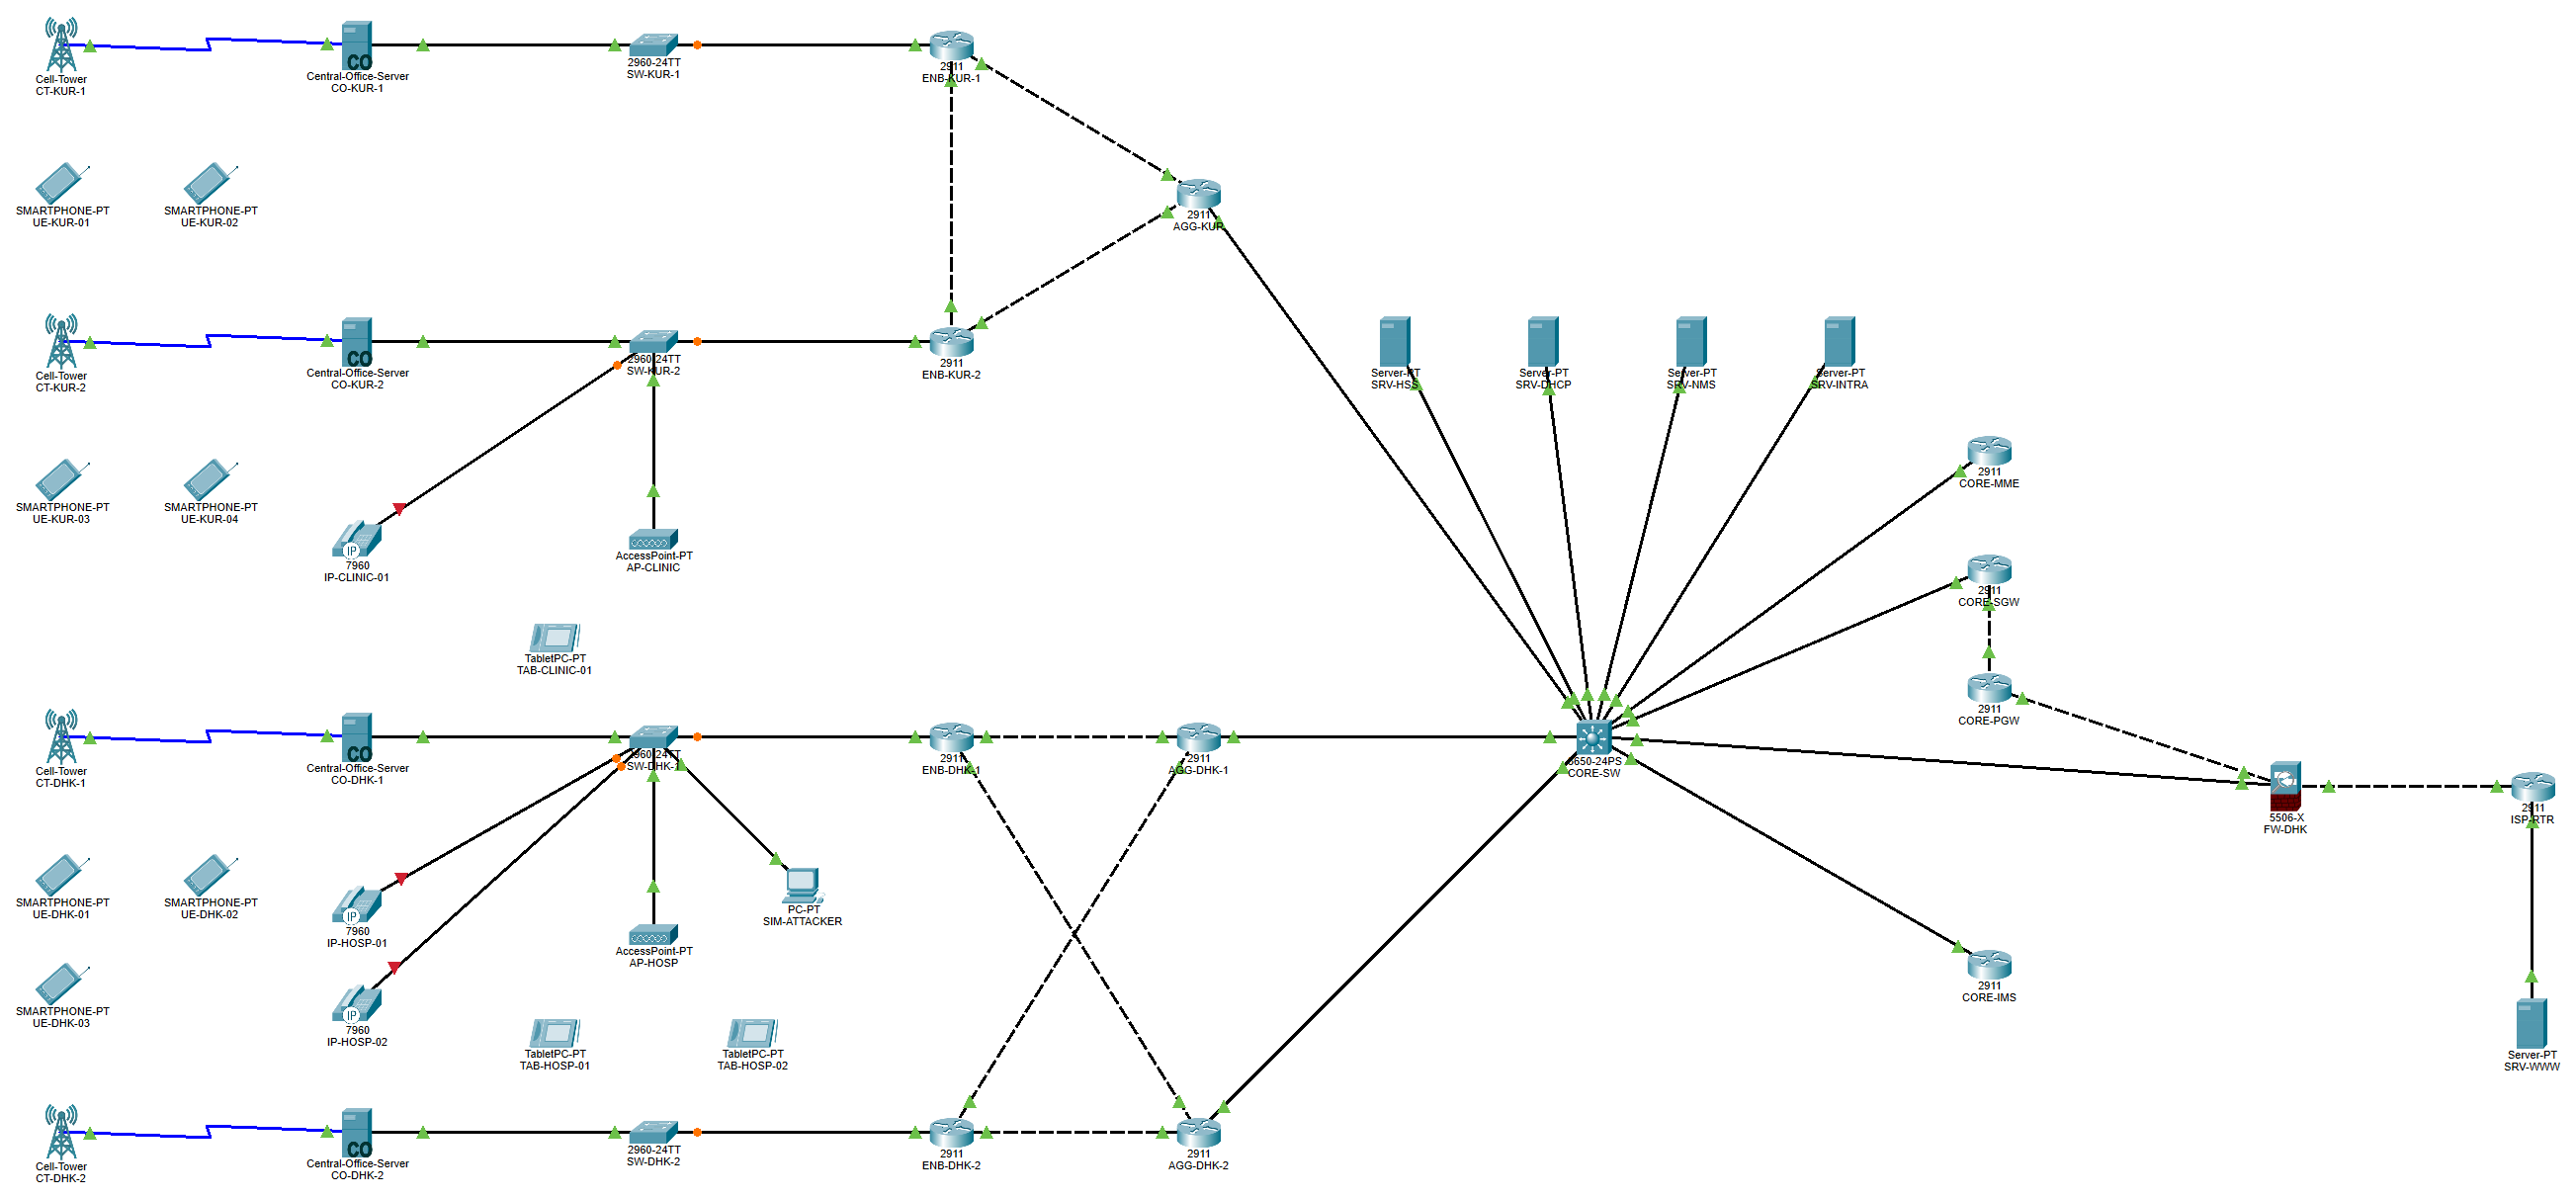
\includegraphics[width=\textwidth]{figures/fig_pt_topology.png}
\caption{Packet Tracer topology: two access rows per area (urban Dhaka, rural Kurigram),
aggregation, and a shared EPC core with HSS, SGW, PGW, MME, IMS, plus firewall and ISP egress.}
\label{fig:pt}
\end{figure}

\subsection{How the model maps onto the design}
The simulator stands in for the radio layer rather than reproducing it. Packet Tracer has no
LTE physical layer, so the four \texttt{Cell-Tower} objects represent the four macro sites of
Table~\ref{tab:budget} (two urban, two rural), and each eNB is backhauled through a
\texttt{2960} access switch and a \texttt{Central-Office-Server} to the aggregation router.
The core follows the same EPC decomposition used in the Q4 and Q7 reasoning: MME for control
plane, SGW/PGW for the user plane, HSS for subscriber data, IMS for VoLTE, and an edge firewall
in front of ISP egress.

\begin{table}[H]\centering\footnotesize
\caption{Device inventory of the Packet Tracer model.}
\label{tab:ptinv}
\begin{tabularx}{\textwidth}{@{}p{5.3cm}p{0.8cm}X@{}}
\toprule
\textbf{Device} & \textbf{Qty} & \textbf{Role in the model} \\
\midrule
\texttt{Cell-Tower} CT-DHK-1/2, CT-KUR-1/2 & 4 & Macro sites, matching the four BDT 6.0 M sites \\
\texttt{2911} eNB-DHK-1/2, eNB-KUR-1/2 & 4 & Baseband/EPC-facing node per site \\
\texttt{2960} SW-DHK-1/2, SW-KUR-1/2 & 4 & Site access switching \\
Central-Office-Server CO-DHK/KUR & 4 & Local service/central-office host \\
\texttt{2911} AGG-DHK-1/2, AGG-KUR & 3 & Aggregation toward the core \\
\texttt{3650} CORE-SW & 1 & Core switch fabric \\
\texttt{2911} CORE-MME/SGW/PGW/IMS & 4 & EPC and IMS functions \\
SRV-HSS/DHCP/NMS/INTRA/WWW & 5 & Subscriber, addressing, management, services \\
\texttt{5505} FW-DHK, \texttt{2911} ISP-RTR & 2 & Security and external egress \\
\texttt{7960} IP-HOSP-01/02, IP-CLINIC-01 & 3 & Hospital and clinic voice terminals \\
AP-HOSP, AP-CLINIC & 2 & Indoor Wi-Fi, standing in for small cells \\
UE-DHK-01..03, UE-KUR-01..04 & 7 & Mobile subscriber endpoints \\
TAB-HOSP-01/02, TAB-CLINIC-01 & 3 & Indoor data clients \\
SIM-ATTACKER & 1 & Traffic generator used to drive load \\
\bottomrule
\end{tabularx}
\end{table}

\subsection{What the model does and does not show}
The capture reproduces the structural claim of Q7, that both areas share one core and one
budget, and it makes the hospital and clinic attachment points explicit. Two qualifications are
recorded. First, the red link indicators on \texttt{IP-HOSP-01}, \texttt{IP-HOSP-02} and
\texttt{IP-CLINIC-01} in Figure~\ref{fig:pt} mark access links that are down,
so continuity of the protected terminals is topology intent, not a passing test. Second, the
BOM small cells appear as Wi-Fi access points, since Packet Tracer models no LTE small cell; no
BER, SINR, reuse or Erlang result here is derived from the simulator, and the numerical results
remain those of Appendices~\ref{app:calc} and~\ref{app:bom}.

% Team contributions: rebalanced allocation requested by the project team.
% This section is a dedicated final page; the technical report above is unchanged.
\clearpage
\section{Team Contributions}
\label{app:team}

The following division of responsibilities reflects the revised allocation
across hardware and budgeting, signal analysis, and network-system planning.
Signal-level results were used as technical inputs to equipment and network
decisions; the responsibilities below identify who led each component.

\vspace{4pt}
\noindent\textbf{Zarif Ahnaf Dhrubo}\hfill\textbf{Student ID: 0812310205101023}\\[-1pt]
\textit{Hardware, power systems, equipment pricing and voice-codec provisioning}
\begin{itemize}[leftmargin=1.5em,topsep=3pt,itemsep=1.5pt,parsep=0pt]
  \item Selected the proposed macro-site, three-sector antenna, indoor small-cell
  and backhaul equipment classes; compiled supporting technical specifications
  and the hardware bill of materials (Q2, Q7 and Appendix B).
  \item Planned 8-hour urban and 24-hour rural backup systems, including the
  battery/solar configuration and hospital--clinic emergency-power provisions
  (Q1 and Q7).
  \item Prepared unit-cost estimates, the BDT 28.8 million base budget,
  contingency and hardware pricing for alternatives and staged upgrades (Q7).
  \item Handled the practical speech-codec comparison and AMR-NB equipment/
  service selection, including PCM-rate and packet-voice overhead considerations
  (coding portion of Q6).
\end{itemize}

\vspace{4pt}
\noindent\textbf{Md. Muhiminul Islam}\hfill\textbf{Student ID: 0812310205101006}\\[-1pt]
\textit{Radio-signal propagation, link budgets, fading and modulation}
\begin{itemize}[leftmargin=1.5em,topsep=3pt,itemsep=1.5pt,parsep=0pt]
  \item Developed the 900/1800 MHz uplink and downlink link budgets, reference
  path-loss calculations, receiver/noise assumptions, indoor margins and
  estimated coverage radii (signal-analysis portion of Q2).
  \item Calculated Doppler shifts and RMS delay spread; examined coherence
  behaviour, BPSK/QPSK BER versus AWGN theory and receiver sensitivity to
  carrier-phase and timing errors (Q3).
  \item Identified signal-quality measurements and supplied propagation/fading
  analysis as technical inputs for diagnosis and the network-design checks
  (supporting Q1, Q4 and Q5).
\end{itemize}

\vspace{4pt}
\noindent\textbf{Khondaokar Miskatul Azim}\hfill\textbf{Student ID: 0812310205101028}\\[-1pt]
\textit{Network architecture, capacity, mobility and integrated evaluation}
\begin{itemize}[leftmargin=1.5em,topsep=3pt,itemsep=1.5pt,parsep=0pt]
  \item Established the urban/rural service objectives and diagnostic approach;
  developed macro-site placement, site-count interpretation, sector layouts,
  frequency-layer assignments and coverage checks (Q1 and layout portion of Q2).
  \item Evaluated frequency reuse, co-channel interference, sectoring,
  busy-hour throughput, backhaul constraints and capacity alternatives (Q4).
  \item Analysed handover traces, hysteresis/time-to-trigger choices and
  dropped-call assessment; dimensioned sector-level voice resources using
  Erlang B (Q5 and traffic portion of Q6).
  \item Integrated the recommended network, compared deployment alternatives,
  tested site failure and traffic growth, and evaluated target compliance,
  stakeholder priorities and the staged plan (Q7).
\end{itemize}

\vspace{4pt}
\begin{table}[H]
\centering\small
\caption{Summary of primary responsibilities by assignment question.}
\begin{tabularx}{\textwidth}{@{}p{1.0cm}>{\raggedright\arraybackslash}p{3.55cm}X@{}}\toprule
\textbf{Q} & \textbf{Primary lead(s)} & \textbf{Assigned work} \\ \midrule
Q1 & Miskatul; Muhiminul; Zarif & Network diagnosis; signal metrics; outage/equipment needs \\
Q2 & Muhiminul; Miskatul; Zarif & Link budgets; site geometry/layout; antenna/equipment inputs \\
Q3 & Muhiminul & Doppler, delay spread, BER and synchronization impairments \\
Q4 & Miskatul (Muhiminul input) & Interference, frequency reuse and capacity planning \\
Q5 & Miskatul (Muhiminul input) & Handover settings, received-signal traces and drop assessment \\
Q6 & Zarif; Miskatul & Speech-codec selection/overhead; Erlang-B voice dimensioning \\
Q7 & Miskatul; Zarif & Final design, stress tests/compliance; hardware, cost and backup \\ \bottomrule
\end{tabularx}
\end{table}

\noindent\textit{Note:} These are responsibility allocations for the group
submission; interdependent decisions were incorporated into the report jointly.

\end{document}
